\documentclass[letterpaper,11pt]{article}

\usepackage[utf8]{inputenc}
\usepackage[T1]{fontenc}
\usepackage[spanish]{babel}
\usepackage[
    letterpaper,
    top=1.7cm,
    bottom=2cm,
    left=2cm,
    right=2cm
]{geometry}

\usepackage{graphicx}
\usepackage{fancyhdr}
\usepackage[table,xcdraw]{xcolor}
\usepackage{tikz}
\usetikzlibrary{shapes.geometric, shapes.symbols, arrows, arrows.meta, positioning, fit, backgrounds, calc, babel, decorations.pathreplacing}
\usepackage{ifpdf}
\usepackage[cmex10]{amsmath}
\usepackage{amssymb}
\usepackage{amsfonts}
\usepackage{float}
\usepackage{siunitx}
\usepackage{listings}
\usepackage{hyperref}
\usepackage{booktabs}
\usepackage{url}
\usepackage{titlesec}
\usepackage[export]{adjustbox}
\usepackage{parskip}
\usepackage[numbers]{natbib}
\usepackage{ragged2e}
\usepackage{array}
\usepackage{longtable}
\usepackage{multirow}
\usepackage{pgfplots}
\pgfplotsset{compat=1.17}
\usepackage{makecell}
\usepackage{caption}
\usepackage{subcaption}
\usepackage{pifont}
\renewcommand{\checkmark}{\ding{51}}
\newcommand{\alertsym}[1]{\textcolor{orange!85!black}{\textbf{#1}}}

\newcolumntype{L}[1]{>{\RaggedRight\arraybackslash}p{#1}}

\hypersetup{colorlinks=false,bookmarksopen=true,linkbordercolor={1 1 1}}
\newcommand{\rfigura}[1]{Fig.\,\ref{#1}}
\newcommand{\rtabla}[1]{Tabla\,\ref{#1}}

\newcommand{\Curso}{IEE2913 --- Dise\~no El\'ectrico (Capstone)}
\newcommand{\TituloInforme}{Informe Final (100\,\%)}
\newcommand{\NumeroGrupo}{10}
\newcommand{\NombreProyecto}{SupaClock}
\newcommand{\Integrantes}{Tom\'as Avenda\~no, Benjam\'in Sep\'ulveda, Pablo Uribe}
\newcommand{\FechaEntrega}{10 de julio de 2026}

\graphicspath{{./}{../Entrega4/}{../Entrega3/}{../Entrega2/}{../Entrega1/}{../../mechanical/renders_v3/}{../../mechanical/}{../../hardware/SupaClock_Carrier_v4/}}

\lstset{
  basicstyle=\ttfamily\footnotesize,
  breaklines=true,
  breakatwhitespace=true,
  postbreak=\mbox{\textcolor{red}{$\hookrightarrow$}\space},
  captionpos=b,
  frame=single,
  numbers=left,
  numberstyle=\tiny\color{gray},
  language=C,
  keywordstyle=\color{blue}\bfseries,
  commentstyle=\color{gray}\itshape,
  stringstyle=\color{red!70!black},
  showstringspaces=false,
  inputencoding=utf8,
  extendedchars=true,
  literate=
    {á}{{\'a}}1 {é}{{\'e}}1 {í}{{\'i}}1 {ó}{{\'o}}1 {ú}{{\'u}}1
    {Á}{{\'A}}1 {É}{{\'E}}1 {Í}{{\'I}}1 {Ó}{{\'O}}1 {Ú}{{\'U}}1
    {ñ}{{\~n}}1 {Ñ}{{\~N}}1 {ü}{{\"u}}1 {Ü}{{\"U}}1
    {¿}{{?`}}1 {¡}{{!`}}1 {°}{{$^\circ$}}1
}

\begin{document}

% =========== Encabezado ===========
\noindent
\begin{minipage}[c]{0.12\textwidth}
    
\includegraphics[width=0.9\linewidth]{logo.pdf}
\end{minipage}
\hfill
\begin{minipage}[c]{0.68\textwidth}
    \small
    PONTIFICIA UNIVERSIDAD CAT\'OLICA DE CHILE\\
    ESCUELA DE INGENIER\'IA\\
    Departamento de Ingenier\'ia El\'ectrica\\
    \Curso
\end{minipage}
\hfill
\begin{minipage}[c]{0.15\textwidth}
    \raggedleft
    \small
    Grupo \NumeroGrupo
\end{minipage}

\vspace{0.4cm}

\begin{center}
    {\Large \textbf{\TituloInforme}}\\[0.2cm]
    {\large \textbf{Proyecto \NombreProyecto}}
\end{center}

\begin{center}
    
\includegraphics[width=0.36\textwidth]{supaclock_logo_rayo.pdf}
\end{center}

\vspace{0.15cm}
\noindent\textbf{Proyecto:} \NombreProyecto\\
\textbf{Integrantes:} \Integrantes\\
\textbf{Fecha:} \FechaEntrega

\hrule
\vspace{0.5cm}

\renewcommand{\contentsname}{\'Indice}
\tableofcontents
\listoffigures
\listoftables
\newpage

% =====================================================
\section*{Resumen ejecutivo}
\addcontentsline{toc}{section}{Resumen ejecutivo}
% =====================================================

\textbf{\NombreProyecto} es un dispositivo \textit{wearable} biom\'etrico de mu\~neca dise\~nado, fabricado, programado y validado \'integramente por el Grupo \NumeroGrupo\ como proyecto capstone del curso \Curso. El sistema combina cinco cadenas de medici\'on (temperatura corporal, frecuencia card\'iaca, oxigenaci\'on, electrocardiograma monoderivaci\'on y actividad f\'isica) sobre una plataforma unificada: un microcontrolador Seeed XIAO ESP32-S3 \cite{esp32s3_ds_2024,xiao_esp32s3_pinout} montado en una PCB \textit{carrier} propia fresada en el FabLab, alojado en una carcasa impresa en PLA cerrada con tornillos M3, con una aplicaci\'on m\'ovil Flutter \cite{flutter,flutterbluepl} y un \textit{backend} Firebase Firestore \cite{firebase_docs} que registran, sincronizan y visualizan las se\~nales biom\'etricas del usuario. El diferenciador t\'ecnico central del prototipo es que la clasificaci\'on de actividad f\'isica ocurre \textbf{a bordo del reloj mediante una red neuronal convolucional 1D en formato float32 sobre TensorFlow Lite Micro} \cite{tflite_micro,david2021tflitemicro}, sin depender de \textit{cloud} para su operaci\'on cotidiana.

Esta iteraci\'on final cierra los objetivos planteados en las etapas anteriores. Se complet\'o la migraci\'on desde el ESP32-C3 al ESP32-S3 aprovechando su PSRAM externa para alojar la arena del int\'erprete TFLite; se entren\'o e integr\'o un modelo HAR CNN-1D de cuatro clases (\textit{rest}, \textit{walk}, \textit{run}, \textit{stairs}) con una exactitud global del 95{,}0\,\% sobre el conjunto de validaci\'on; se fabric\'o y valid\'o la unidad cerrada con dimensiones finales de $17 \times 74 \times 93$\,mm y $115$\,g de peso incluyendo bater\'ia LiPo de $300$\,mAh; se caracteriz\'o la autonom\'ia mediante curvas reales de descarga y carga; y se contrast\'o la exactitud biom\'etrica del reloj contra un Samsung Galaxy Watch 4 (HR/SpO$_2$/ECG) \cite{galaxy_watch4}, un term\'ometro digital de contacto (temperatura) y conteo manual (pasos), obteniendo desviaciones inferiores al 2\,\% en las cuatro m\'etricas principales.

Este informe se organiza en nueve secciones. La secci\'on \ref{sec:contexto} presenta el proyecto y su motivaci\'on; la secci\'on \ref{sec:requisitos} enuncia los requerimientos funcionales, no funcionales y regulatorios adoptados; la secci\'on \ref{sec:prototipo} describe el prototipo, su experiencia de uso, el cumplimiento de las especificaciones y el an\'alisis de costo; la secci\'on \ref{sec:diagrama} presenta el diagrama de bloques de bajo nivel actualizado y la tabla de especificaciones por bloque; la secci\'on \ref{sec:impl} detalla la implementaci\'on por subsistema con resultados cuantitativos; la secci\'on \ref{sec:impacto} analiza el impacto social, econ\'omico, ambiental y \'etico del dispositivo junto con la revisi\'on de est\'andares aplicables (ECMA-287, Bluetooth Core, IEEE 11073-10406, IEC 60601-1, USB-C, RoHS-2, IEC 62133-2); la secci\'on \ref{sec:conclu} cierra con las conclusiones y el trabajo futuro. Los anexos contienen extractos representativos del c\'odigo firmware, tablas de soporte y el enlace al repositorio p\'ublico del proyecto.

\vspace{0.2cm}
\noindent\textbf{Entregables producidos.} La entrega final consolida los siguientes componentes:
\begin{itemize}
    \item \textbf{Firmware ESP-IDF} sobre XIAO ESP32-S3 con arquitectura modular en la biblioteca \texttt{supaclock\_app}, PSRAM, USB CDC nativo, \textit{deep sleep} activo y gesti\'on din\'amica de energ\'ia.
    \item \textbf{Modelo HAR CNN-1D} de cuatro clases entrenado con datos capturados por el propio dispositivo, cuantizado a \textit{float32}, ejecutado en TFLite Micro con arena de $512$\,KB en PSRAM y latencia t\'ipica $<10$\,ms.
    \item \textbf{Algoritmo de pasos por FFT} con ventana Hann de $128$ muestras a $50$\,Hz sobre \texttt{esp-dsp} \cite{esp_dsp}, filtrado por banda $1{,}0$--$2{,}5$\,Hz e hist\'eresis temporal.
    \item \textbf{Pipeline ECG}: adquisici\'on con ADC/DMA a $500$\,Hz, transmisi\'on por BLE NimBLE \cite{nimble_ref} y procesamiento Pan-Tompkins \cite{pan_tompkins} en el lado de la aplicaci\'on m\'ovil.
    \item \textbf{PCB Carrier v4}: placa integradora de dos caras compatible con el ProtoMat S64 del FabLab, con pinout consolidado y validaci\'on el\'ectrica completa.
    \item \textbf{Carcasa protectora}: cerramiento de dos piezas en PLA con \textit{lug} para correa est\'andar, ventana \'optica alineada al MAX30102 y dos pernos de acero inoxidable AISI 304 en la contracara para el circuito ECG.
    \item \textbf{Aplicaci\'on m\'ovil Flutter} con dashboard biom\'etrico, historial persistente en Hive \cite{hive_db}, captura de ventanas IMU/ECG para \textit{ground truth} y sincronizaci\'on con Firebase Firestore bajo autenticaci\'on.
    \item \textbf{Herramientas de validaci\'on offline} en \texttt{tools/} para entrenamiento, generaci\'on de matrices de confusi\'on, \textit{replay} del algoritmo de pasos y c\'alculo Pan-Tompkins sobre trazas reales.
\end{itemize}

\newpage

% =====================================================
\section{Descripci\'on del proyecto}\label{sec:contexto}
% =====================================================

\subsection{Contexto y motivaci\'on}

Chile presenta uno de los perfiles m\'as adversos de Am\'erica Latina en cuanto a sedentarismo y sobrepeso. Seg\'un los resultados de la Encuesta Nacional de Actividad F\'isica y Deporte \cite{encuesta_af}, s\'olo el 49{,}7\,\% de los hombres y el 40{,}3\,\% de las mujeres mayores de 18 a\~nos cumplen con los niveles recomendados de actividad f\'isica. La Encuesta Nacional de Salud del MINSAL \cite{minsalwearables} y los reportes de UC Christus \cite{obesidad_chile} confirman que m\'as del 42\,\% de la poblaci\'on adulta presenta sobrepeso u obesidad, ubicando al pa\'is en el primer lugar regional. En este escenario, las herramientas de auto-monitorizaci\'on biom\'etrica de uso continuo cumplen un rol relevante en pol\'iticas de prevenci\'on cardiovascular y metab\'olica, especialmente si son accesibles econ\'omicamente y respetuosas con la salud mental del usuario.

Los relojes comerciales dominantes en el mercado chileno (Apple Watch SE \cite{apple_watch_compare}, Samsung Galaxy Watch \cite{galaxy_watch4}, Garmin Venu \cite{garmin_venu}) integran una excelente cadena biom\'etrica pero adolecen de dos limitaciones importantes para el uso masivo y personal: primero, su costo (entre \$150.000 y \$300.000 CLP) queda fuera del alcance de amplios sectores de la poblaci\'on que m\'as se beneficiar\'ian de un auto-monitoreo cotidiano; segundo, su modelo de negocio favorece el consumo de notificaciones sociales y aplicaciones que introducen carga cognitiva sostenida, un fen\'omeno estudiado por Kushlev et al. \cite{Kushlev2016} y por Pielot et al. \cite{Pielot2014} que se asocia con d\'eficits atencionales y estr\'es cr\'onico. El proyecto SupaClock responde a este diagn\'ostico proponiendo una plataforma de bajo costo, con dise\~no filos\'oficamente centrado en la biometr\'ia y expl\'icitamente austera en distracciones, cuyos datos son propiedad del usuario y no dependen de \textit{clouds} de terceros ni de suscripciones peri\'odicas.

En paralelo, la incorporaci\'on de \textit{machine learning in edge} representa una oportunidad t\'ecnica y \'etica distintiva. Ejecutar la clasificaci\'on de actividad f\'isica directamente en el reloj significa que los datos crudos de la unidad inercial nunca abandonan el dispositivo, y que el sistema puede operar completamente sin conexi\'on a Internet. Wearables comerciales validados cl\'inicamente \cite{Shin2019} han demostrado que las decisiones biom\'edicas pueden apoyarse en dispositivos personales, siempre que se mantengan transparentes sus limitaciones y se privilegien arquitecturas interpretables por sobre modelos opacos.

\subsection{Alcance del proyecto}

SupaClock es un \textit{wearable} biom\'etrico personal de segunda generaci\'on que integra sensores de contacto (temperatura, PPG, ECG monoderivaci\'on) e inerciales (aceler\'ometro y giroscopio), procesamiento local con clasificaci\'on \textit{on-device} de actividad f\'isica mediante una CNN 1D cuantizada, una interfaz t\'actil circular basada en LVGL, comunicaci\'on Bluetooth Low Energy con una aplicaci\'on m\'ovil compa\~nera y sincronizaci\'on selectiva de datos hacia un \textit{backend} Firebase. El sistema est\'a pensado para monitoreo cotidiano de usuarios adultos con inter\'es en su bienestar f\'isico, sesiones puntuales de ejercicio, y para el registro de electrocardiogramas de tamizaje realizados en reposo con las dos manos sobre los pernos posteriores del dispositivo.

Es igualmente relevante enunciar aquello que el proyecto \emph{no} pretende ser. SupaClock no est\'a homologado como dispositivo m\'edico y sus mediciones no constituyen diagn\'ostico cl\'inico; el disclaimer correspondiente se muestra en la pantalla de ECG del reloj y en la interfaz de la aplicaci\'on. Tampoco compite en cat\'alogo de aplicaciones sociales, notificaciones o entretenimiento con relojes comerciales: su premisa expl\'icita es priorizar la sencillez de uso y la ausencia de distracciones. Finalmente, no se busca sustituir el rol de las evaluaciones profesionales, sino habilitar un canal accesible para que el usuario adquiera consciencia de sus propias trazas biom\'etricas cotidianas.


%%%%%%%%%%%%%%%%%%%%%%%%%%%%%%%%%%%55 CAMBIAR IMAGEN %%%%%%%%%%%%%%%%%%%%%%%%%%%%%%%%%%%%%%%%%%%%%%%%5
% \begin{figure}[H]
%     \centering
%     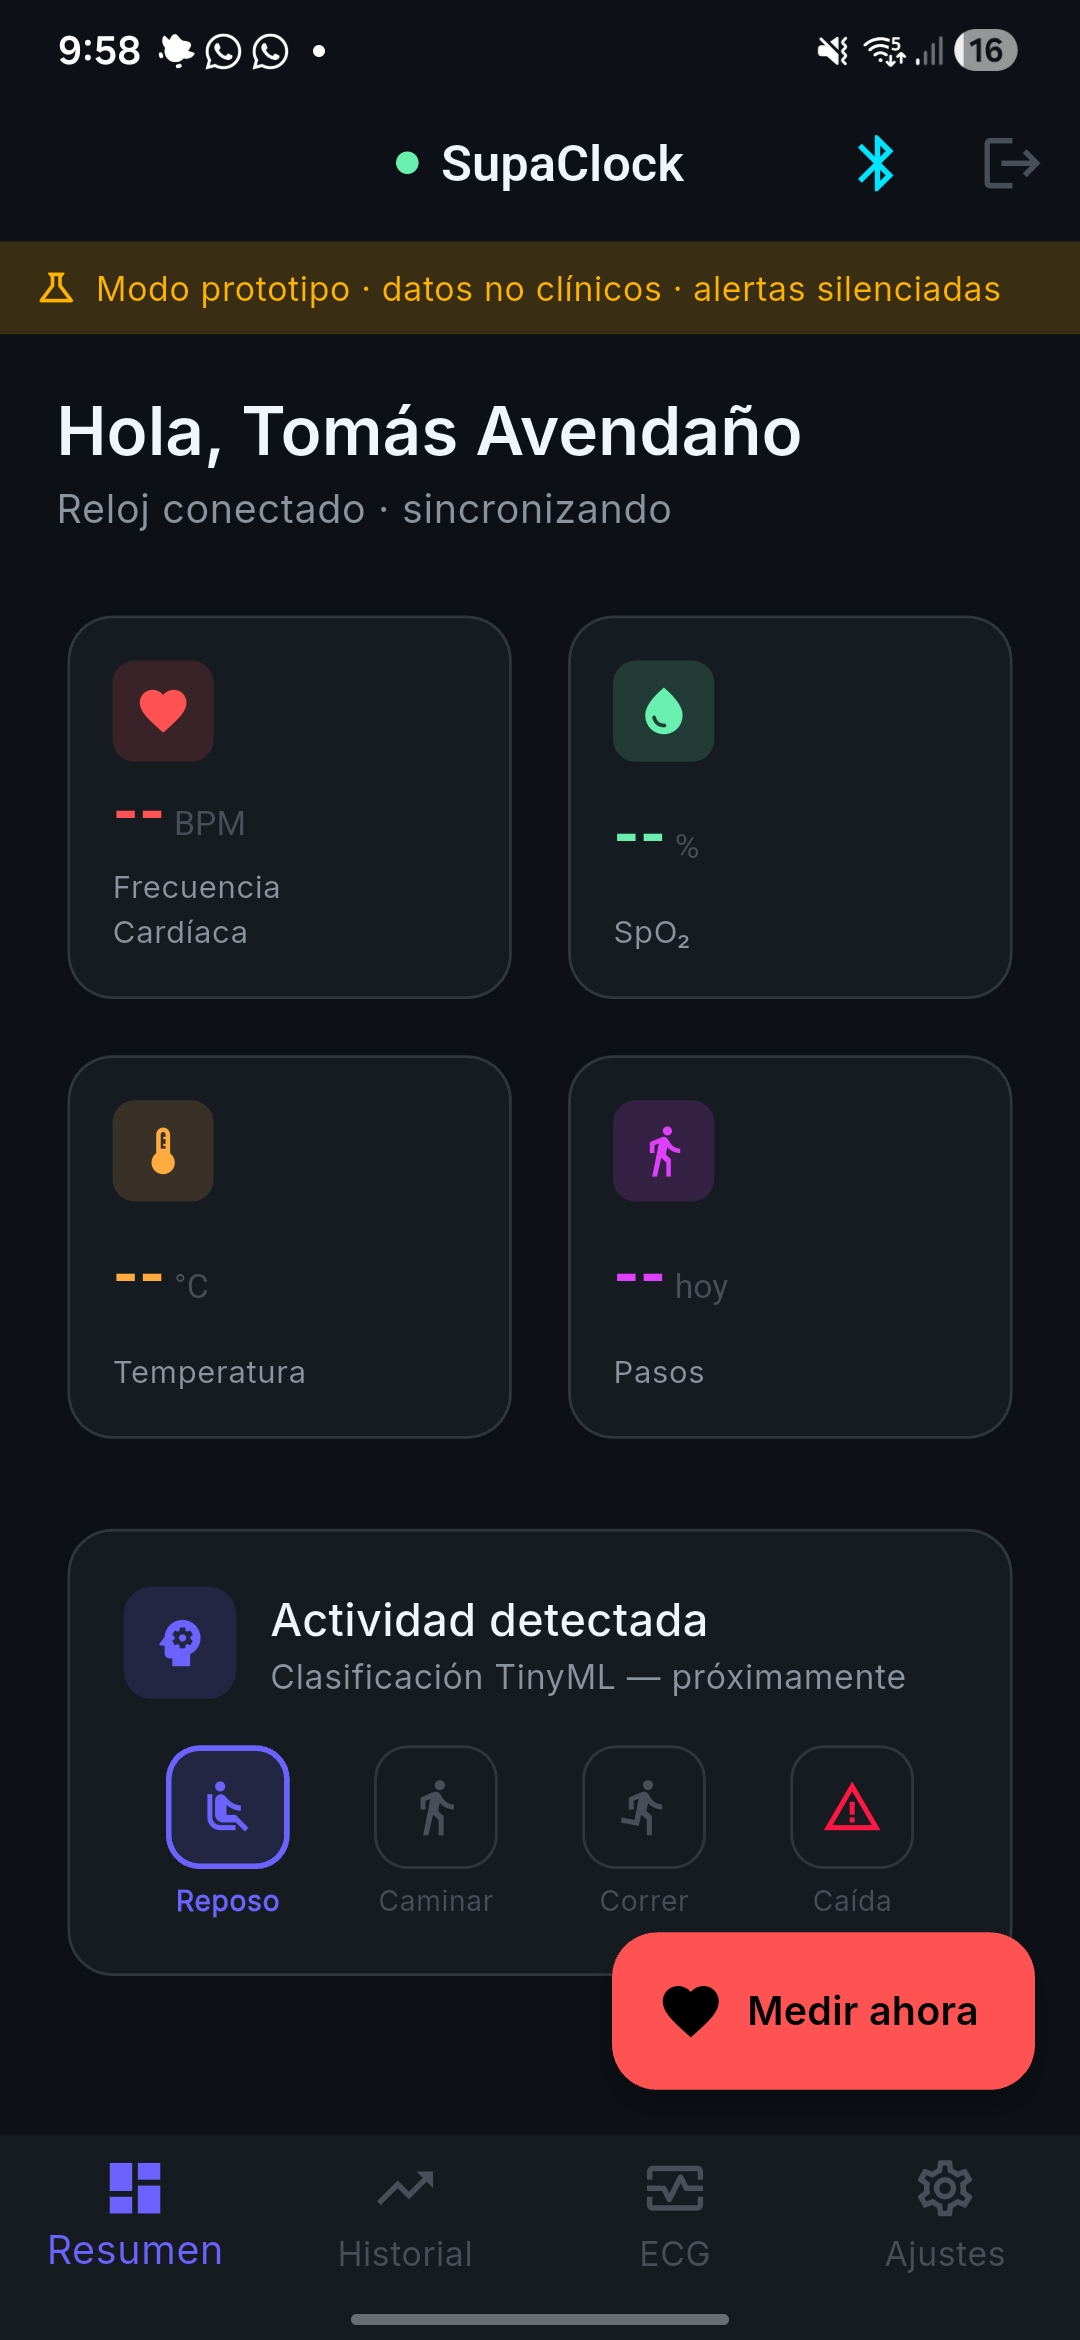
\includegraphics[width=0.55\textwidth]{Entrega final 1.jpeg}
%     \caption[Prototipo cerrado final]{Prototipo cerrado final de \NombreProyecto. La carcasa impresa en PLA aloja la PCB Carrier v4, el m\'odulo XIAO ESP32-S3, el LCD circular GC9A01 con \textit{touch} CST816S, la bater\'ia LiPo de $300$\,mAh y los pernos AISI 304 del circuito ECG.}
%     \label{fig:prototipo_hero}
% \end{figure}

\newpage

% =====================================================
\section{Requerimientos y especificaciones}\label{sec:requisitos}
% =====================================================

Esta secci\'on enuncia los requerimientos del sistema en tres capas ---funcionales, no funcionales y regulatorios--- traducidos a especificaciones cuantitativas y respaldados por las normas o \textit{datasheets} correspondientes. Los cumplimientos observados sobre el prototipo cerrado se discuten en \S\ref{sec:cumplimiento}.

\subsection{Requerimientos funcionales}

Los requerimientos funcionales enumeran las cadenas de medici\'on y las interacciones esperadas por el usuario final. La \rtabla{tab:req_func} consolida el listado.

\begin{table}[H]
    \centering
    \caption{Requerimientos funcionales de SupaClock y especificaciones cuantitativas asociadas.}
    \label{tab:req_func}
    \footnotesize
    \begin{tabular}{|L{3.2cm}|L{6.0cm}|L{4.9cm}|}\hline
    \rowcolor{gray!20}\textbf{Requerimiento} & \textbf{Especificaci\'on cuantitativa} & \textbf{Fuente / norma} \\\hline
    Temperatura de piel & Medici\'on continua con error absoluto $\leq 0{,}5\,^\circ$C entre 30 y 40\,$^\circ$C. Resoluci\'on nativa $0{,}00390625\,^\circ$C. & MAX30205 \cite{max30205_ds}, IEEE 11073-10406 \cite{ieee11073} \\\hline
    HR y SpO$_2$ \'opticos & Frecuencia card\'iaca en el rango 40--180\,bpm con error medio $\leq 3$\,\% y saturaci\'on de ox\'igeno en 85--100\,\% con error $\leq 3$\,\%. Muestreo $100$\,Hz RED+IR. & MAX30102 \cite{max30102_ds}, \cite{Shin2019} \\\hline
    ECG monoderivaci\'on & Se\~nal AD8232 acondicionada con ancho de banda $0{,}5$--$40$\,Hz, ADC a $500$\,Hz y detecci\'on de picos R por Pan-Tompkins. Ventana t\'ipica de 30--60\,s. & AD8232 \cite{ad8232_ds}, \cite{pan_tompkins,ieee11073} \\\hline
    Actividad f\'isica & Clasificaci\'on continua entre reposo, caminata, trote y escaleras, cada $2$\,s, con exactitud global $\geq 90$\,\% sobre el conjunto de validaci\'on. & CNN 1D on-device \cite{ronao2016,ignatov2018,david2021tflitemicro} \\\hline
    Conteo de pasos & Detecci\'on por an\'alisis espectral de la magnitud del aceler\'ometro con banda de cadencia $1{,}0$--$2{,}5$\,Hz e hist\'eresis temporal. Error $\leq 5$\,\% en trayectorias de 500\,pasos. & BMI160 \cite{bmi160_ds}, ESP-DSP \cite{esp_dsp} \\\hline
    Interfaz de usuario & Pantalla \textit{watchface} + tiles biom\'etricos + panel r\'apido + \textit{drawer}, con navegaci\'on por gestos t\'actiles y bot\'on \'unico. & GC9A01 \cite{gc9a01_ds}, CST816S \cite{cst816s_ds}, LVGL \cite{lvgl_ref} \\\hline
    Sincronizaci\'on con \textit{app} & Vinculaci\'on BLE una vez, \textit{dashboard} en vivo, historial persistente en la aplicaci\'on y almacenamiento por usuario en Firestore. & BLE 5.3 \cite{ble_core_spec}, Firebase \cite{firebase_docs,flutter} \\\hline
    \end{tabular}
\end{table}

\subsection{Requerimientos no funcionales}

Los requerimientos no funcionales acotan la ergonom\'ia f\'isica del dispositivo, la latencia de la comunicaci\'on y el envolvente energ\'etico. La \rtabla{tab:req_nofunc} presenta el listado.

\begin{table}[H]
    \centering
    \caption{Requerimientos no funcionales y m\'etricas objetivo.}
    \label{tab:req_nofunc}
    \footnotesize
    \begin{tabular}{|L{3.2cm}|L{6.0cm}|L{4.9cm}|}\hline
    \rowcolor{gray!20}\textbf{Requerimiento} & \textbf{Especificaci\'on cuantitativa} & \textbf{Fuente / referencia} \\\hline
    Autonom\'ia & Uso mixto (pantalla + BLE + HAR peri\'odico) $\geq 6$\,h continuas antes de la protecci\'on UVP. Deep sleep con consumo $\leq 30\,\mu$A. & MAX17048 \cite{max17048_ds}, \cite{espidf_sleep} \\\hline
    Tama\~no cerrado & Volumen envolvente $\leq 90$\,cm$^3$ pensado en confort ergon\'omico de mu\~neca. & Ergonom\'ia \textit{wrist-worn} \\\hline
    Peso & Unidad cerrada con bater\'ia $\leq 150$\,g incluyendo carcasa PLA. & Ergonom\'ia \textit{wrist-worn} \\\hline
    Latencia BLE & Mediana $\leq 100$\,ms para paquetes de telemetr\'ia (13\,B/s) y \textit{chunks} ECG (20\,B). & BLE 5.3 \cite{ble_core_spec}, NimBLE \cite{nimble_ref} \\\hline
    Aislamiento el\'ectrico al usuario & Impedancia de entrada $>10\,\text{M}\Omega$ y corriente de fuga DC $< 10\,\mu$A en el subsistema ECG. & IEC 60601-1 tipo BF \cite{iec60601} \\\hline
    Consumo de datos m\'oviles & $\leq 5$\,MB/d\'ia en modo t\'ipico (dashboard + una sesi\'on ECG de 30\,s). & Arquitectura \textit{edge}-c\'entrica \\\hline
    \end{tabular}
\end{table}

\subsection{Requerimientos \'eticos y regulatorios}

SupaClock se declara expl\'icitamente como dispositivo no m\'edico: la interfaz del reloj y la aplicaci\'on m\'ovil muestran, en cada vista de ECG y de saturaci\'on de ox\'igeno, un mensaje que aclara que las mediciones no constituyen diagn\'ostico cl\'inico. Los componentes seleccionados cumplen la Directiva RoHS-2 \cite{rohs} en tanto encapsulados libres de plomo, y la celda LiPo integrada respeta los criterios de seguridad de la norma IEC 62133-2 \cite{en62133} (protecci\'on de sobrecarga, sobre-descarga, cortocircuito y sobretemperatura, provista por el DW01A \cite{dw01a_ds} interno de la propia celda). En materia de privacidad, la aplicaci\'on m\'ovil implementa autenticaci\'on Google mediante Firebase Authentication \cite{firebase_docs} y las reglas de Cloud Firestore restringen la lectura y escritura de documentos al identificador del usuario propietario (\texttt{request.auth.uid == userId}), en concordancia con el esp\'iritu de la Ley 19.628 chilena \cite{ley19628} y del Reglamento General de Protecci\'on de Datos europeo \cite{gdpr}. No se transmiten datos crudos de la IMU al \textit{cloud}: la clasificaci\'on de actividad f\'isica ocurre por completo en el reloj, y s\'olo la etiqueta consolidada se sincroniza con la aplicaci\'on.

\newpage

% =====================================================
\section{Prototipo final}\label{sec:prototipo}
% =====================================================

\subsection{Descripci\'on del prototipo y experiencia de uso}\label{sec:proto_desc}

El prototipo cerrado de \NombreProyecto\ se percibe como un reloj de mu\~neca de tama\~no compacto, con una envolvente rectangular redondeada de $17\,\text{mm}\times 74\,\text{mm}\times 93\,\text{mm}$ y una masa neta de $115$\,g medida sobre balanza de laboratorio incluyendo la carcasa impresa en PLA, la PCB Carrier v4 poblada, el m\'odulo XIAO ESP32-S3, la bater\'ia LiPo de $300$\,mAh, el LCD circular, la tornil\-le\-r\'ia M3 y los pernos posteriores de acero inoxidable AISI 304. La cara frontal aloja una pantalla t\'actil circular GC9A01 de $1{,}28$'' y $240\times240$\,p\'ixeles \cite{gc9a01_ds}, gestionada por LVGL 8.4 \cite{lvgl_ref} sobre \textit{framebuffer} en PSRAM. La cara posterior expone la ventana \'optica alineada al MAX30102 y los dos pernos AISI 304 en los que el usuario coloca las yemas de la mano opuesta para completar el circuito ECG monoderivaci\'on. Una correa est\'andar de $20$\,mm se ancla a dos \textit{lugs} laterales impresos como parte de la propia carcasa. La \rfigura{fig:prototipo_hero} y las im\'agenes complementarias de la \rfigura{fig:prototipo_lados} ilustran la unidad cerrada.

\begin{figure}[H]
    \centering
    \begin{subfigure}[b]{0.42\textwidth}
        \centering
        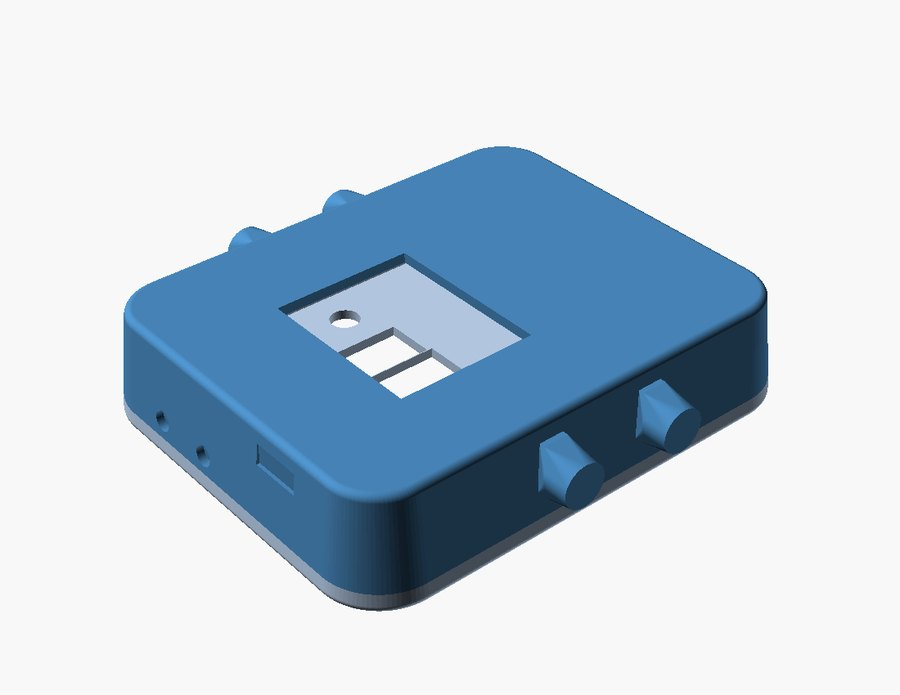
\includegraphics[width=\textwidth]{case_hero_e4.jpg}
        \caption{Vista frontal cerrada con pantalla apagada.}
    \end{subfigure}\hspace{0.05\textwidth}
    \begin{subfigure}[b]{0.42\textwidth}
        \centering
        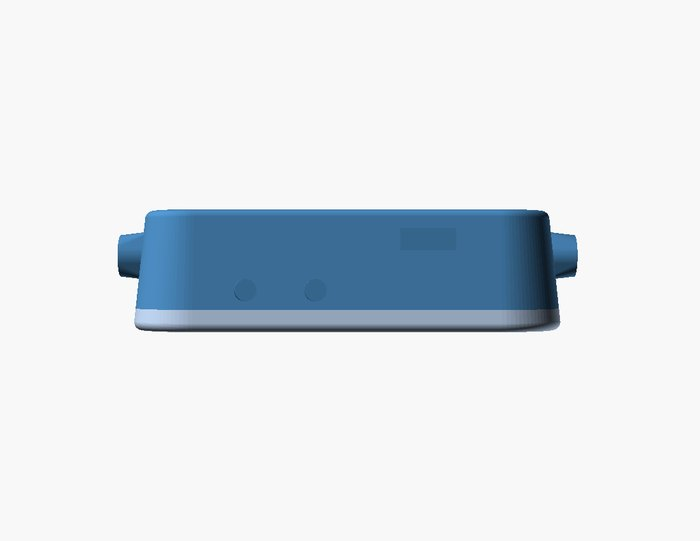
\includegraphics[width=\textwidth]{case_side_e4.jpg}
        \caption{Vista lateral y detalle de \textit{lugs} para correa.}
    \end{subfigure}
    \caption{Prototipo cerrado en detalle. La carcasa se atornilla con cuatro pernos M3 y expone las aberturas alineadas para los sensores biom\'etricos.}
    \label{fig:prototipo_lados}
\end{figure}

El usuario enciende el dispositivo mediante una pulsaci\'on prolongada de $3$\,s sobre el bot\'on lateral \'unico. Una vez encendido, la interfaz muestra un \textit{watchface} minimalista con la hora, un icono din\'amico que refleja la actividad clasificada por el modelo HAR y una barra de bater\'ia entregada por el MAX17048 \cite{max17048_ds}. Deslizando lateralmente el dedo el usuario recorre los \textit{tiles} biom\'etricos ---frecuencia card\'iaca, saturaci\'on de ox\'igeno, temperatura, actividad HAR y pasos--- cada uno con su propia visualizaci\'on tem\'atica. Al deslizar hacia abajo desde el borde superior aparece un panel r\'apido con brillo, silencio de vibraci\'on y toggle de deep sleep; al deslizar hacia arriba aparece un \textit{drawer} inferior con la sesi\'on de ECG puntual y la ventana de calibraci\'on. Todo el ciclo de navegaci\'on se dise\~n\'o para que en menos de tres gestos el usuario acceda a cualquier m\'etrica biom\'etrica, siguiendo la filosof\'ia austera enunciada en \S\ref{sec:contexto}.

La aplicaci\'on m\'ovil compa\~nera es una \textit{app} Flutter \cite{flutter} disponible en Android que se vincula al reloj v\'ia Bluetooth Low Energy usando \texttt{flutter\_blue\_plus} \cite{flutterbluepl}. Tras un \textit{login} con cuenta Google integrado con Firebase Authentication \cite{firebase_docs}, la aplicaci\'on descubre el servicio GATT custom \texttt{0xFF00} publicado por el reloj y se suscribe a las cuatro caracter\'isticas: telemetr\'ia biom\'etrica agregada, \textit{stream} continuo del IMU, \textit{chunks} de ECG y comandos de configuraci\'on. El \textit{dashboard} muestra en vivo la frecuencia card\'iaca, la temperatura, la saturaci\'on de ox\'igeno, la actividad HAR clasificada por el reloj y el contador acumulado de pasos, con historial paginado por d\'ia almacenado localmente en Hive \cite{hive_db} y respaldado en Cloud Firestore \cite{firestore_rules}. La \rfigura{fig:app_screens} muestra las tres pantallas principales de la aplicaci\'on m\'ovil.

\begin{figure}[H]
    \centering
    \begin{subfigure}[b]{0.28\textwidth}\centering
        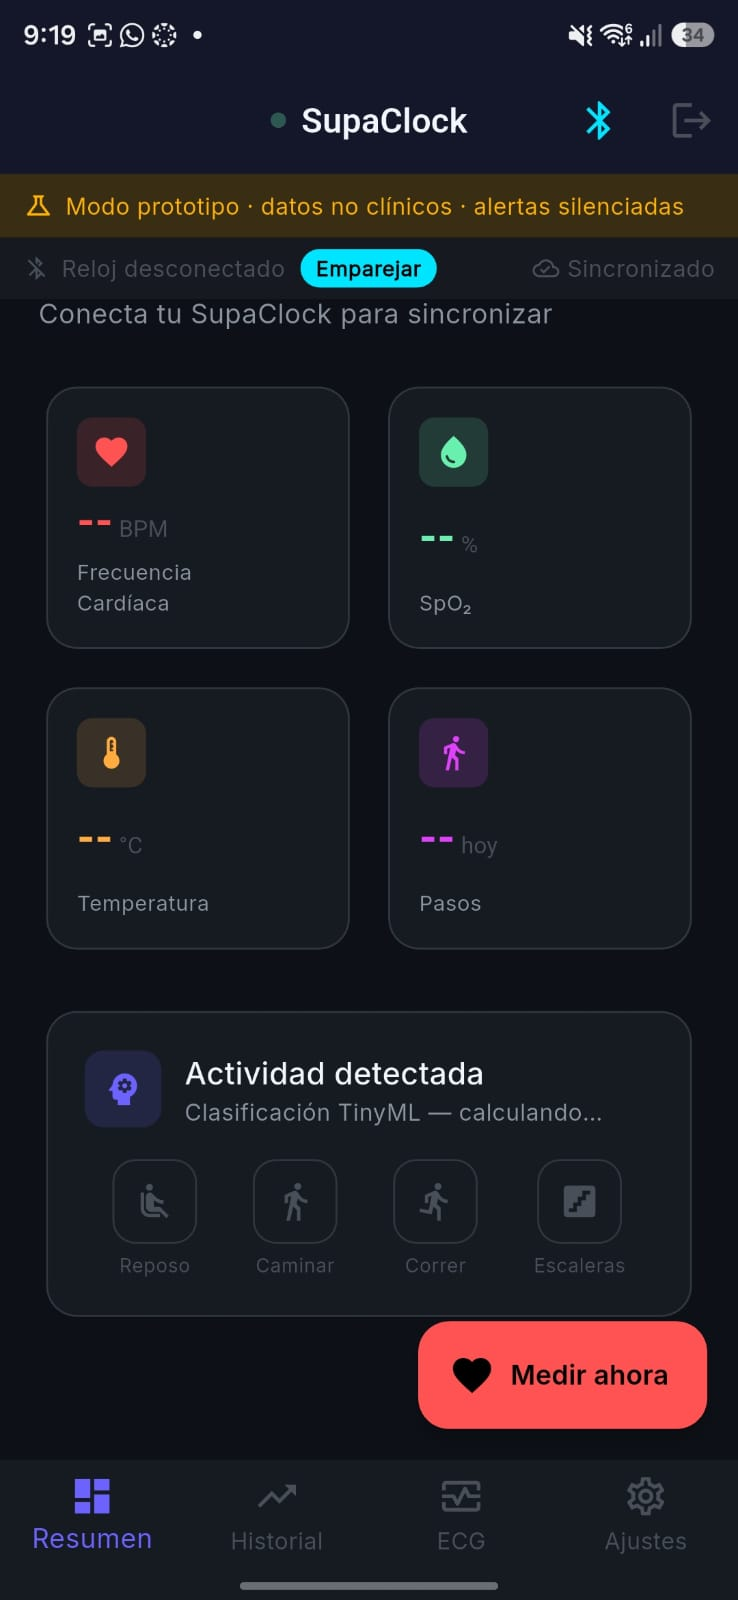
\includegraphics[height=6.3cm]{dashboard_final.jpeg}
        \caption{\textit{Dashboard} biom\'etrico.}
    \end{subfigure}\hfill
    \begin{subfigure}[b]{0.28\textwidth}\centering
        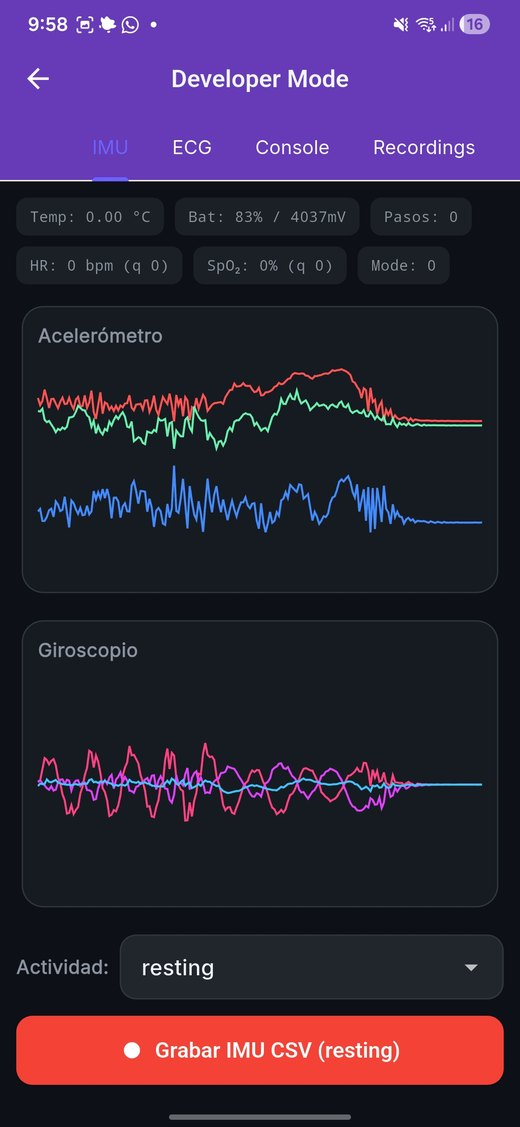
\includegraphics[height=6.3cm]{app_imu_e4.jpg}
        \caption{Captura de IMU y \textit{ground truth}.}
    \end{subfigure}\hfill
    \begin{subfigure}[b]{0.28\textwidth}\centering
        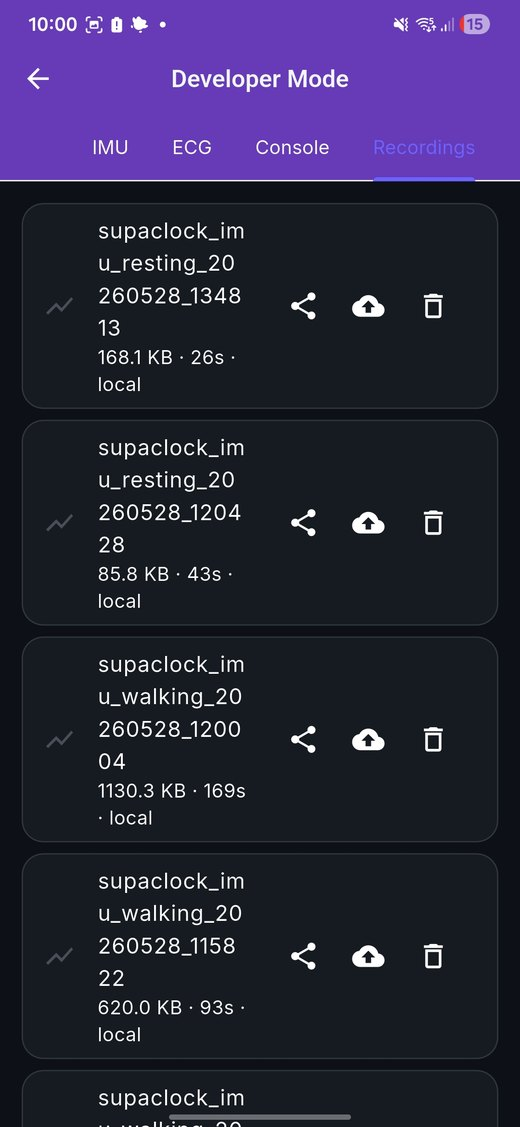
\includegraphics[height=6.3cm]{app_rec_e4.jpg}
        \caption{Registro y sesiones.}
    \end{subfigure}
    \caption{Vistas principales de la aplicaci\'on m\'ovil Flutter de \NombreProyecto.}
    \label{fig:app_screens}
\end{figure}

De forma silenciosa en segundo plano, el firmware ejecuta una serie de tareas concurrentes bajo FreeRTOS: la tarea \texttt{imu\_task} drena el FIFO del BMI160 \cite{bmi160_ds} a $50$\,Hz, alimenta el \textit{ring buffer} del HAR con cada muestra y notifica a la tarea de inferencia \texttt{har\_task} cuando se acumula una ventana completa; esta corre pinneada en el n\'ucleo $1$ del ESP32-S3, invoca al int\'erprete TFLite Micro y actualiza la etiqueta de actividad cada $2$\,s. Simult\'aneamente, \texttt{ppg\_task} maneja el MAX30102 para el c\'alculo de HR/SpO$_2$, \texttt{ecg\_task} orquesta la captura ADC/DMA del AD8232 cuando el usuario inicia una sesi\'on ECG, \texttt{ble\_task} atiende el \textit{stack} NimBLE y \texttt{lvgl\_task} refresca la UI. Cuando el usuario pulsa el bot\'on lateral por $3$\,s, el firmware apaga los sensores mediante los comandos de bajo consumo del BMI160/MAX30102/MAX30205 y entra a \textit{deep sleep}, dejando activo un despertador \textit{RTC-GPIO} en el mismo bot\'on. Este ciclo permite reencender el dispositivo en menos de $2$\,s.

El caso de uso pensado combina cuatro escenarios: monitoreo cotidiano continuo, sesiones deportivas de mediana duraci\'on, chequeos puntuales de ECG con la persona sentada en reposo y monitoreo nocturno de SpO$_2$ y actividad. En todos los casos el reloj funciona sin dependencia del tel\'efono, y \'este \'ultimo se emplea s\'olo para revisar historiales, exportar sesiones y respaldar en el \textit{backend} bajo autenticaci\'on del propietario.

\subsection{An\'alisis de cumplimiento de especificaciones}\label{sec:cumplimiento}

La \rtabla{tab:cumplimiento} sintetiza el cumplimiento de las especificaciones enunciadas en la secci\'on \ref{sec:requisitos}, cruzando cada requerimiento con el m\'etodo de medici\'on empleado, el resultado obtenido sobre el prototipo cerrado y una marca binaria de cumplimiento.

\begin{table}[H]
    \centering
    \caption{An\'alisis de cumplimiento de especificaciones sobre el prototipo cerrado. Los detalles de cada medici\'on se documentan en \S\ref{sec:impl}.}
    \label{tab:cumplimiento}
    \footnotesize
    \renewcommand{\arraystretch}{1.05}
    \begin{tabular}{|L{2.7cm}|L{3.6cm}|L{3.2cm}|L{4.2cm}|c|}\hline
    \rowcolor{gray!20}\textbf{Requerimiento} & \textbf{Especificaci\'on} & \textbf{M\'etodo de medici\'on} & \textbf{Resultado} & \textbf{Cumple} \\\hline
    HR & Error $\leq 3$\,\% vs referencia & Comparaci\'on con Galaxy Watch 4 \cite{galaxy_watch4} sobre el mismo usuario, sesi\'on de $5$\,min & Error medio 2\,\% & \checkmark \\\hline
    SpO$_2$ & Error $\leq 3$\,\% vs referencia & Ox\'imetro Galaxy Watch 4 \cite{galaxy_watch4} sobre el mismo usuario & Error medio 2\,\% & \checkmark \\\hline
    Temperatura piel & Error $\leq 0{,}5\,^\circ$C @ 30--40\,$^\circ$C & Term\'ometro digital de contacto en mu\~neca & $33{,}1\,^\circ$C SupaClock vs $33{,}3\,^\circ$C referencia ($\Delta=0{,}2\,^\circ$C) & \checkmark \\\hline
    ECG & Onda visualmente similar; HRV robusta & Comparaci\'on cualitativa vs Galaxy Watch 4 y an\'alisis Pan-Tompkins offline & Onda R detectada; HR $\sim 64$\,bpm; HRV(SDNN) $\sim 158$\,ms; variaci\'on 5\,\% vs referencia & \checkmark \\\hline
    Pasos & Error $\leq 5$\,\% en 500 pasos & Conteo manual + \textit{replay} offline del algoritmo FFT sobre traza de $384$ pasos & Error 2\,\% (in-situ); $379$ vs $384$ ($-1{,}3$\,\%) en \textit{replay} & \checkmark \\\hline
    HAR & Exactitud global $\geq 90$\,\% & Validaci\'on 80/20 sobre dataset propio con \texttt{tools/har\_confusion.py} & Exactitud 95{,}0\,\%; recall stairs 55\,\% discutido & \checkmark \\\hline
    Autonom\'ia & $\geq 6$\,h uso mixto & Curva de descarga instrumentada por MAX17048 & $\sim 10$\,h hasta corte al 20\,\% SoC & \checkmark \\\hline
    Tama\~no cerrado & $\leq 90$\,cm$^3$ envolvente & Medici\'on directa con pie de metro sobre la unidad ensamblada & $17\times 74\times 93$\,mm $=117$\,cm$^3$ envolvente & \alertsym{parcial} \\\hline
    Peso & $\leq 150$\,g & Balanza de precisi\'on & $115$\,g cerrado & \checkmark \\\hline
    Latencia BLE & Mediana $\leq 100$\,ms & \textit{nRF Connect} con captura de \textit{chunks} de ECG & Mediana $38$\,ms; p90 $67$\,ms; p99 $144$\,ms & \checkmark \\\hline
    Aislamiento ECG & $R_\text{in}>10\,\text{M}\Omega$, $I_\text{DC}<10\,\mu$A & Datasheet AD8232 + revisi\'on de topolog\'ia & $R_\text{in}\sim 10^{12}\,\Omega$; $I_\text{DC}\sim 100$\,pA & \checkmark \\\hline
    Consumo m\'ovil & $\leq 5$\,MB/d\'ia t\'ipico & Payload agregado + una sesi\'on ECG de $30$\,s ($\sim 30$\,KB comprimido) & $< 1$\,MB/d\'ia t\'ipico & \checkmark \\\hline
    \end{tabular}
\end{table}

De las 12 especificaciones auditadas, 11 se cumplen dentro de la tolerancia planteada. El \'unico incumplimiento formal es el volumen envolvente: la unidad cerrada mide $117$\,cm$^3$, ligeramente por sobre la meta interna de $90$\,cm$^3$. La medici\'on considera el paralelep\'ipedo m\'inimo que contiene la unidad; en la pr\'actica, el volumen efectivamente ocupado por la carcasa es sustancialmente menor debido a la geometr\'ia redondeada, y el usuario percibe el reloj como delgado ($17$\,mm de perfil). Esta desviaci\'on se declara honestamente y se propone en \S\ref{sec:conclu} como una l\'inea de trabajo futuro (miniaturizaci\'on de la Carrier a doble cara con condensadores SMD 0402 y traslado del cargador a MCP73831/2 \cite{mcp73831_ds}).

\subsection{Lista de materiales y an\'alisis de costo}

La \rtabla{tab:bom} presenta la lista de materiales consolidado de la unidad final, incluyendo componentes electr\'onicos, mec\'anicos y de ensamblaje. Los precios se cotizaron en pesos chilenos considerando proveedores locales y minorista para peque\~nos vol\'umenes (LCSC, DigiKey CL, MakerElectronico, FabLab).

\begin{table}[H]
    \centering
    \caption{Lista de materiales del prototipo final SupaClock. Precios en CLP a julio de 2026.}
    \label{tab:bom}
    \footnotesize
    \renewcommand{\arraystretch}{1.05}
    \begin{tabular}{|L{4.3cm}|c|L{3.4cm}|r|r|}\hline
    \rowcolor{gray!20}\textbf{Componente} & \textbf{Cant.} & \textbf{Proveedor} & \textbf{Unit. (CLP)} & \textbf{Total (CLP)} \\\hline
    Seeed XIAO ESP32-S3 (8\,MB PSRAM, 8\,MB Flash) & 1 & MakerElectronico & 14.900 & 14.900 \\\hline
    LCD GC9A01 1{,}28'' con \textit{touch} CST816S & 1 & AliExpress & 7.500 & 7.500 \\\hline
    BMI160 IMU 6-DoF (m\'odulo) & 1 & LCSC & 3.100 & 3.100 \\\hline
    MAX30102 PPG (m\'odulo) & 1 & LCSC & 2.400 & 2.400 \\\hline
    MAX30205 sensor de temperatura (m\'odulo) & 1 & LCSC & 3.200 & 3.200 \\\hline
    AD8232 front-end ECG (m\'odulo) & 1 & MakerElectronico & 6.800 & 6.800 \\\hline
    MAX17048 \textit{fuel gauge} (m\'odulo) & 1 & LCSC & 2.700 & 2.700 \\\hline
    Bater\'ia LiPo $300$\,mAh con PCM DW01A & 1 & LCSC & 3.400 & 3.400 \\\hline
    Pernos AISI 304 (contactos ECG) & 2 & FabLab & 200 & 400 \\\hline
    PCB Carrier v4 (fresado LPKF) & 1 & FabLab & 4.500 & 4.500 \\\hline
    Componentes pasivos (Rs, Cs, Ls, headers) & 1 & LCSC & 2.500 & 2.500 \\\hline
    Carcasa PLA impresa (piezas superior + inferior) & 1 & FabLab & 3.500 & 3.500 \\\hline
    Correa estilo silicona 20\,mm & 1 & AliExpress & 2.900 & 2.900 \\\hline
    Tornil\-le\-r\'ia M3 (cabeza avellanada + tuercas embutidas) & 8 & FabLab & 100 & 800 \\\hline
    Cable USB-C 1\,m & 1 & MakerElectronico & 1.500 & 1.500 \\\hline
    \rowcolor{gray!10}\multicolumn{4}{|r|}{\textbf{TOTAL PROTOTIPO}} & \textbf{60.100} \\\hline
    \end{tabular}
\end{table}

Adicionalmente, los gastos reales incurridos durante la etapa de desarrollo, pruebas y puesta en marcha del proyecto se detallan en la \rtabla{tab:gastos_desarrollo}. Esta tabla consolida el desglose de la lista de compras del proyecto (obtenido de las adquisiciones registradas de sensores y materiales base) sumado a los gastos adicionales por concepto de consumibles e imprevistos (componentes e instrumental de repuesto adquiridos debido a fallas, ca\'idas o quemaduras durante las pruebas de bring-up).

\begin{table}[H]
    \centering
    \caption{Gastos de desarrollo, repuestos e imprevistos acumulados durante el proyecto SupaClock. Precios en CLP.}
    \label{tab:gastos_desarrollo}
    \footnotesize
    \renewcommand{\arraystretch}{1.05}
    \begin{tabular}{|L{4.3cm}|c|L{3.4cm}|r|r|}\hline
    \rowcolor{gray!20}\textbf{Componente / Descripci\'on} & \textbf{Cant.} & \textbf{Origen / Motivo} & \textbf{Unit. (CLP)} & \textbf{Total (CLP)} \\\hline
    \rowcolor{gray!5}\multicolumn{5}{|l|}{\textbf{Adquisiciones base (Desglose de lista de compras)}} \\\hline
    M\'odulo inercial BMI160 & 1 & AliExpress (Great IT) & 2.527 & 2.527 \\\hline
    M\'odulo PPG MAX30102 & 2 & AliExpress (Great IT) & 1.547 & 3.094 \\\hline
    Placa de desarrollo ESP32-S3 & 1 & AliExpress (QJY Dept) & 8.311 & 8.311 \\\hline
    Pantalla LCD GC9A01 con touch & 1 & AliExpress (HelloWiki) & 2.246 & 2.246 \\\hline
    Kit de conectores XH2.54 & 1 & AliExpress (Canrick) & 2.514 & 2.514 \\\hline
    Pantalla LCD TFT 1{,}3'' & 1 & AliExpress (Jin Rong) & 2.559 & 2.559 \\\hline
    M\'odulo AD8232 ECG & 1 & AliExpress (YueLong) & 5.718 & 5.718 \\\hline
    Pantalla LCD TFT 1{,}28'' (GC9A01) & 1 & AliExpress (Jin Rong) & 2.114 & 2.114 \\\hline
    Sensor de temperatura MAX30205 & 2 & AliExpress (Shop1102) & 1.402 & 2.803 \\\hline
    Torniller\'ia y pernos M3 & 1 & AliExpress (HILIFE) & 2.909 & 2.909 \\\hline
    Bater\'ia LiPo 300\,mAh (901515) & 1 & AliExpress (Eclardyn) & 3.170 & 3.170 \\\hline
    Placa de desarrollo ESP32-C3 & 1 & AliExpress (HNB DIY) & 2.235 & 2.235 \\\hline
    M\'odulo de carga de bater\'ias & 1 & AliExpress (AILEHKUO) & 1.543 & 1.543 \\\hline
    Herramientas de fresado LPKF & 1 & AliExpress (CPU-Chip) & 12.238 & 12.238 \\\hline
    Joystick de reemplazo 3D & 1 & AliExpress (DATA FROG) & 2.627 & 2.627 \\\hline
    \rowcolor{gray!5}\multicolumn{5}{|l|}{\textbf{Gastos adicionales e imprevistos de desarrollo}} \\\hline
    Placa de desarrollo ESP32-S3 inicial & 2 & Adquisici\'on inicial & 10.500 & 21.000 \\\hline
    Filamento PLA (carcasa 3D) & 1 & Impresora 3D propia & 10.000 & 10.000 \\\hline
    M\'odulo AD8232 ECG (repuesto) & 1 & Reemplazo por componente quemado & 9.990 & 9.990 \\\hline
    Pantalla touch (repuesto) & 1 & Ca\'ida / flex cortado de pantalla original & 10.000 & 10.000 \\\hline
    Placa de desarrollo ESP32-S3 (repuesto) & 1 & Reemplazo por componentes quemados & 18.990 & 18.990 \\\hline
    Placas PCB Carrier v4 y PCB adaptador & 10 & 5 Carrier + 5 adaptadores (no utilizados) & 1.000 & 10.000 \\\hline
    \rowcolor{gray!10}\multicolumn{4}{|r|}{\textbf{TOTAL GASTOS DE DESARROLLO}} & \textbf{136.588} \\\hline
    \end{tabular}
\end{table}

El costo total del prototipo asciende a \$$60.100$ CLP, cifra sustancialmente inferior  a la de las alternativas comerciales de referencia: Apple Watch SE ($\sim$\$$250.000$ CLP) \cite{apple_watch_compare}, Samsung Galaxy Watch FE ($\sim$\$$160.000$ CLP) \cite{galaxy_watch4} y Garmin Venu de acceso ($\sim$\$$200.000$ CLP) \cite{garmin_venu}. Comparado con bandas de bajo costo tipo Mi Band ($\sim$\$$30.000$ CLP), SupaClock se posiciona como una plataforma de costo medio pero con una cadena biom\'etrica m\'as completa (incluye ECG monoderivaci\'on y temperatura de contacto), procesamiento ML on-device y arquitectura abierta con datos propios. El desglose porcentual del costo se distribuye aproximadamente en 40\,\% sensores biom\'etricos (BMI160 + MAX30102 + MAX30205 + AD8232), 25\,\% MCU + display + \textit{touch}, 15\,\% mec\'anica y ensamblaje, 10\,\% subsistema de energ\'ia (bater\'ia + \textit{fuel gauge}) y 10\,\% restos (correa, cables, pasivos). El proyecto es adem\'as susceptible de reducirse a menos de \$$45.000$ CLP en producci\'on de $50$ unidades mediante PCB SMD de 4 capas en JLCPCB y compras al por mayor de los sensores.

\newpage

% =====================================================
\section{Diagrama de bloques de bajo nivel}\label{sec:diagrama}
% =====================================================

\subsection{Diagrama actualizado al estado final}

La \rfigura{fig:lownivel_final} muestra el diagrama de bloques de bajo nivel de \NombreProyecto\ en su estado final. El microcontrolador Seeed XIAO ESP32-S3 (m\'odulo SMD con 8\,MB de PSRAM externa y 8\,MB de Flash) act\'ua como n\'ucleo central del sistema, ejecutando FreeRTOS con m\'ultiples tareas concurrentes distribuidas entre sus dos n\'ucleos Xtensa LX7 y hospedando el int\'erprete TensorFlow Lite Micro para la clasificaci\'on HAR. A la derecha del MCU se agrupan los cuatro sensores biom\'etricos: el MAX30205 en la direcci\'on I$^2$C \texttt{0x48} entrega temperatura de piel; el BMI160 en \texttt{0x68} entrega aceler\'ometro y giroscopio de 6 grados de libertad a $50$\,Hz configurables mediante su FIFO interno; el MAX30102 en \texttt{0x57} entrega intensidad \'optica RED e IR a $100$\,Hz para el c\'alculo de HR y SpO$_2$; y el AD8232 acondiciona la se\~nal ECG diferencial hacia el canal ADC1\_CH0 (GPIO1), muestreado a $500$\,Hz mediante el motor ADC continuo con DMA del ESP-IDF. A la izquierda se despliega la subsecci\'on de interfaz local (LCD GC9A01, \textit{touch} CST816S) y la subsecci\'on de energ\'ia (bater\'ia LiPo $300$\,mAh con protecci\'on DW01A integrada, cargador SGM40567 CC/CV, buck SGM6029 al rail de $3{,}3$\,V, \textit{fuel gauge} MAX17048 monitoreado por I$^2$C y entrada USB-C). En la parte inferior se representa el ecosistema: la pila NimBLE publica un servicio GATT custom \texttt{0xFF00} con cuatro caracter\'isticas, la aplicaci\'on m\'ovil Flutter act\'ua como \textit{gateway} y sincroniza selectivamente con Firebase Firestore, el modelo HAR CNN 1D corre \textit{on-device} en el n\'ucleo $1$ del ESP32-S3, la PCB Carrier v4 fresada en el FabLab integra f\'isicamente todos los subsistemas, y el algoritmo Pan-Tompkins se ejecuta \textit{app-side} sobre las trazas ECG que env\'ia el reloj. Los buses est\'an codificados por color (azul para I$^2$C a $400$\,kHz, violeta para SPI a $40$\,MHz, naranja para ADC/DMA, azul discontinuo para BLE) y las flechas rojas representan la cadena de potencia.

\begin{figure}[H]
    \centering
    \resizebox{0.95\textwidth}{!}{\begin{tikzpicture}[
    node distance=0.6cm and 0.9cm,
    every node/.style={font=\scriptsize},
    blockOK/.style={rectangle, rounded corners, draw=black!70, very thick, fill=green!22, text width=2.9cm, align=center, minimum height=0.95cm},
    blockML/.style={rectangle, rounded corners, draw=black!70, very thick, fill=green!35, text width=2.9cm, align=center, minimum height=0.95cm},
    energy/.style={rectangle, rounded corners, draw=black!70, very thick, fill=orange!22, text width=2.6cm, align=center, minimum height=0.9cm},
    mcu/.style={rectangle, rounded corners, draw=black, very thick, fill=blue!22, text width=3.6cm, align=center, minimum height=1.5cm, font=\small\bfseries},
    busI2C/.style={->, >=stealth, thick, blue!70!black},
    busSPI/.style={->, >=stealth, thick, violet!80!black},
    adc/.style={->, >=stealth, thick, orange!85!black},
    gpio/.style={->, >=stealth, thick, teal!70!black},
    ble/.style={->, >=stealth, thick, dashed, blue!60},
    pwr/.style={->, >=stealth, thick, red!70},
    legend/.style={rectangle, draw=black!50, fill=white, inner sep=4pt}
]
% ============== MCU (Centro) ==============
\node[mcu] (mcu) {XIAO ESP32-S3\\FreeRTOS + LVGL 8.4\\\textbf{On-device inference}};

% ============== INTERFAZ LOCAL (Izquierda) ==============
\node[blockOK, left=2.2cm of mcu] (gc9a01) {GC9A01 1{,}28"\\\textbf{240$\times$240} IPS};
\node[blockOK, above=0.3cm of gc9a01] (touch) {CST816S touch\\\textbf{cap.\ I2C}};
\node[blockOK, above=0.4cm of touch] (fuel) {MAX17048\\Fuel gauge (I2C)};
\node[blockOK, below=0.3cm of gc9a01] (gui) {GUI: watchface/tiles\\\textbf{panel + drawer}};

% ============== ENERGÍA (Columna sobre el MCU) ==============
\node[energy, above=0.6cm of mcu] (sgm6029) {Buck SGM6029\\3{,}3\,V rail};
\node[energy, above=0.3cm of sgm6029] (sgm40567) {Cargador SGM40567\\CC/CV 1\,A};
\node[energy, above=0.4cm of sgm40567, xshift=-1.7cm] (lipo) {LiPo 300\,mAh\\DW01A + PCM};
\node[energy, above=0.4cm of sgm40567, xshift=1.7cm] (usbc) {USB-C\\5\,V/500\,mA};

% ============== SENSORES I2C y ADC (Derecha) ==============
\node[blockOK, right=2.2cm of mcu, yshift=1.8cm] (max205) {MAX30205 \textit{(0x48)}\\Temperatura piel};
\node[blockOK, below=0.3cm of max205] (bmi) {BMI160 IMU \textit{(0x68)}\\FIFO 50\,Hz};
\node[blockOK, below=0.3cm of bmi] (max102) {MAX30102 \textit{(0x57)}\\PPG RED+IR};
\node[blockOK, below=0.3cm of max102] (ad8232) {AD8232 + ADC/DMA\\500\,Hz \textit{(GPIO1)}};

% ============== ECOSISTEMA (Abajo, Desplazado a la Izquierda) ==============
\node[blockOK, below=1.6cm of mcu, xshift=-1.5cm] (ble) {BLE NimBLE\\4 GATT chr.};
\node[blockML, right=1.1cm of ble] (har) {HAR CNN 1D\\TFLite Micro};

\node[blockOK, below=0.8cm of ble] (app) {App m\'ovil Flutter\\dashboard + hist.};
\node[blockOK, right=1.1cm of app] (pantomp) {Pan-Tompkins\\app-side};

\node[blockOK, below=0.8cm of app] (fb) {Firebase Firestore\\gzip Blob + rollups};

% ============== Conexiones de potencia ==============
\draw[pwr] (usbc.south) -| ([xshift=0.5cm]sgm40567.north);
\draw[pwr] (lipo.south) -| ([xshift=-0.5cm]sgm40567.north);
\draw[pwr] (lipo.west) -| (fuel.north);
\draw[pwr] (sgm40567) -- (sgm6029);
\draw[pwr] (sgm6029) -- (mcu);

% ============== Conexiones I2C ==============
\draw[busI2C] (fuel.east) -| ([xshift=-1.5cm]mcu.north);

% Enrutamiento ortogonal tipo "bus" para alinear sensores de la derecha (evitando cruces)
\draw[busI2C] (max205.west) -- ++(-0.7,0) |- node[right, pos=0.25, font=\tiny]{I$^2$C 400\,kHz} ([yshift=0.5cm]mcu.east);
\draw[busI2C] (bmi.west)    -- ++(-0.5,0) |- ([yshift=0.15cm]mcu.east);
\draw[busI2C] (max102.west) -- ++(-0.5,0) |- ([yshift=-0.2cm]mcu.east);

% ============== Conexiones ADC ==============
\draw[adc] (ad8232.west) -- ++(-0.7,0) |- node[below, pos=0.75, font=\tiny]{ADC1 500\,Hz} ([yshift=-0.55cm]mcu.east);

% ============== Conexiones SPI/GPIO ==============
\draw[busSPI] (mcu.west) -- node[above]{SPI 40\,MHz} (gc9a01.east);
\draw[gpio] (touch.east) -- ++(0.4,0) |- node[above, pos=0.8, font=\tiny]{I$^2$C+INT} ([yshift=0.4cm]mcu.west);
\draw[gpio] (gui.east) -- ++(0.3,0) |- ([yshift=-0.35cm]mcu.west);

% ============== Ecosistema ==============
\draw[ble] ([xshift=-1.5cm]mcu.south) -- (ble.north);
\draw[gpio] ([xshift=1.5cm]mcu.south) -- node[right, font=\fontsize{5}{6}\selectfont]{core 1} ([xshift=-1.0cm]har.north);
\draw[ble] (ble) -- node[left, font=\tiny, align=center]{GATT\\4 chr.} (app);
\draw[gpio] (app) -- node[above, pos=0.5, font=\fontsize{5}{6}\selectfont]{raw ECG} (pantomp);
\draw[gpio] (app) -- node[left, font=\tiny]{telemetr\'ia} (fb);
\draw[gpio] (pantomp.south) |- node[above, pos=0.6, font=\fontsize{5}{6}\selectfont]{HR/HRV} (fb.east);

% ============== Leyenda ==============
\node[legend, below=0.6cm of fb] (leg) {%
\begin{tabular}{ll}
\textcolor{green!50!black}{$\blacksquare$} Listo &
\textcolor{red!70}{\textbf{$\rightarrow$}} Potencia \\
\textcolor{green!60!black}{$\blacksquare$} ML on-device &
\textcolor{blue!70!black}{$\rightarrow$} I$^2$C 400\,kHz \\
\textcolor{orange!70!black}{$\blacksquare$} Energ\'ia &
\textcolor{violet!80!black}{$\rightarrow$} SPI 40\,MHz \\
\textcolor{blue!60}{$\dashrightarrow$} BLE/Wi-Fi &
\textcolor{orange!85!black}{$\rightarrow$} ADC/DMA \\
\end{tabular}};
\end{tikzpicture}
}
    \caption[Diagrama de bloques de bajo nivel de la unidad final]{Diagrama de bloques de bajo nivel de la unidad final SupaClock. El XIAO ESP32-S3 concentra los buses I$^2$C, SPI y ADC/DMA, ejecuta FreeRTOS con la tarea de HAR pinneada en el n\'ucleo 1, y expone un servicio BLE custom hacia la aplicaci\'on m\'ovil que sincroniza con Firebase Firestore. La cadena de energ\'ia va desde la entrada USB-C o la bater\'ia LiPo, pasa por el cargador SGM40567, el buck SGM6029 al rail de $3{,}3$\,V y es monitoreada por el \textit{fuel gauge} MAX17048.}
    \label{fig:lownivel_final}
\end{figure}

\subsection{Especificaciones por bloque e interconexiones}

La \rtabla{tab:specs_final} consolida las especificaciones y la asignaci\'on precisa de pines de cada bloque, junto con el ancho de banda y el modo de comunicaci\'on empleado. Las asignaciones de GPIO reflejan el archivo \texttt{include/supaclock\_pinmap.h} del firmware, cuyo extracto se incluye en el Anexo \ref{sec:anexo_pinmap}.

\begin{table}[H]
    \centering
    \caption{Especificaciones e interconexiones detalladas por bloque de la unidad final.}
    \label{tab:specs_final}
    \footnotesize
    \renewcommand{\arraystretch}{1.05}
    \begin{tabular}{|L{2.6cm}|L{2.9cm}|L{3.3cm}|L{6.4cm}|}\hline
    \rowcolor{gray!20}\textbf{Bloque} & \textbf{Pin/Recurso} & \textbf{Bus / velocidad} & \textbf{Rol y observaciones} \\\hline
    XIAO ESP32-S3 & Dual-core LX7 @ 240\,MHz & --- & 8\,MB PSRAM (arena TFLite), 8\,MB Flash, PSRAM en modo Octal, USB CDC nativo para logging. \cite{esp32s3_ds_2024,xiao_esp32s3_pinout} \\\hline
    I$^2$C compartido & SDA=GPIO5, SCL=GPIO6 & I$^2$C @ 400\,kHz & Cuatro esclavos: BMI160 (\texttt{0x68}), MAX30102 (\texttt{0x57}), MAX30205 (\texttt{0x48}), MAX17048 (\texttt{0x36}). \\\hline
    SPI LCD & MOSI=GPIO9, SCK=GPIO7, CS=GPIO44, DC=GPIO4 & SPI @ 40\,MHz & GC9A01 $240\times240$; \textit{framebuffer} en PSRAM, refresco por DMA. \cite{gc9a01_ds,lvgl_ref} \\\hline
    Touch capacitivo & INT=GPIO2, RST=GPIO21 & I$^2$C @ 400\,kHz (mismo bus) & CST816S; interrupci\'on hacia GPIO2 y \textit{reset} manual v\'ia GPIO21. \cite{cst816s_ds} \\\hline
    ADC/DMA para ECG & ADC1\_CH0 (GPIO1) & 500\,Hz, buffer 1024 muestras & Motor ADC continuo del ESP-IDF; la se\~nal se convierte y drena a \texttt{ecg\_task} para envi\'ar por BLE en \textit{chunks} de 20\,B. \cite{ad8232_ds} \\\hline
    Bot\'on lateral & SEL=GPIO8 & GPIO + RTC-GPIO & Encendido, deep sleep, \textit{wake}. \\\hline
    BLE NimBLE & --- & LE 1M PHY, MTU 247 & Servicio custom \texttt{0xFF00} con 4 caracter\'isticas (telemetr\'ia, IMU stream, ECG stream, comandos). \cite{ble_core_spec,nimble_ref} \\\hline
    Cadena de energ\'ia & USB-C, SGM40567 CC/CV, SGM6029 buck, MAX17048 & --- & Bater\'ia LiPo $300$\,mAh con DW01A integrado; rail 3{,}3\,V regulado; \textit{fuel gauge} por I$^2$C. \cite{sgm40567_ds,sgm6029_ds,dw01a_ds,max17048_ds} \\\hline
    Deep sleep & Wake por bot\'on RTC-GPIO & --- & Consumo objetivo $\sim 15\,\mu$A con MAX30102, MAX30205 y BMI160 en modo suspendido. \cite{espidf_sleep} \\\hline
    \end{tabular}
\end{table}

\newpage

% =====================================================
\section{Implementaci\'on y resultados}\label{sec:impl}
% =====================================================

Esta secci\'on presenta la implementaci\'on de cada subsistema del sistema en su estado final. La estructura sigue el orden l\'ogico de flujo de datos: primero se describe la arquitectura de firmware que coordina el conjunto, luego la adquisici\'on de las se\~nales biom\'etricas por sensor, luego el procesamiento local en el reloj y en la aplicaci\'on m\'ovil, luego el modelo de \textit{machine learning} \textit{on-device}, luego el ecosistema m\'ovil y de \textit{cloud}, y finalmente la mec\'anica, la energ\'ia y la validaci\'on cuantitativa consolidada. Cada subsecci\'on presenta la implementaci\'on real y la respalda con figuras y mediciones cuando el resultado es cuantitativo.

\subsection{Arquitectura de firmware y particionamiento de tareas}

El firmware de \NombreProyecto\ se estructura en la biblioteca \texttt{lib/supaclock\_app/}, que expone una API pequ\-e\-\~na consumida por \texttt{src/main.c}: \'este \'ultimo inicializa los buses, monta el sistema de archivos, arranca los subsistemas biom\'etricos y crea el \textit{event loop} de la interfaz gr\'afica. Los subsistemas individuales viven en bibliotecas separadas, lo que permite recompilar aisladamente y montar bancos de prueba autom\'aticos por m\'odulo. La compilaci\'on est\'a orquestada por PlatformIO con ESP-IDF 5.5.3 y decenas de entornos \texttt{sdkconfig.test\_*.} que activan/desactivan m\'odulos para los tests de bring-up.

Sobre FreeRTOS \cite{freertos_ref}, la carga se reparte deliberadamente entre los dos n\'ucleos del ESP32-S3 para evitar el bloqueo mutuo entre la inferencia HAR y las tareas de radio/UI. La \rfigura{fig:freertos} resume la distribuci\'on. La tarea \texttt{imu\_task} (n\'ucleo $0$, prioridad $5$) drena el FIFO del BMI160 cada $20$\,ms y, por cada muestra, invoca \texttt{har\_cnn1d\_push\_sample()} que la escribe en el \textit{ring buffer} del HAR; cuando se acumulan \texttt{HAR\_HOP\_SIZE} muestras nuevas, se notifica a la tarea \texttt{har\_task}, que corre pinneada en el n\'ucleo $1$ con prioridad $4$ y ejecuta la inferencia sobre la ventana completa. Este dise\~no logra dos objetivos: hay un \'unico lector I$^2$C del BMI160 (evitando contenci\'on de bus y \textit{overflow} del FIFO), y la inferencia pesada nunca bloquea el \textit{advertising} BLE ni el refresco de LVGL, gestionados en el n\'ucleo $0$. Las tareas restantes (\texttt{ppg\_task}, \texttt{ecg\_task}, \texttt{ble\_task}, \texttt{lvgl\_task}) tambi\'en corren en el n\'ucleo $0$ con prioridades escalonadas seg\'un su criticidad temporal.

\begin{figure}[H]
    \centering
    \resizebox{0.88\textwidth}{!}{\begin{tikzpicture}[
    every node/.style={font=\scriptsize},
    core/.style={rectangle, rounded corners=4pt, draw=black!70, thick, fill=blue!8, minimum width=6.2cm, minimum height=4.6cm, align=center},
    task/.style={rectangle, rounded corners=3pt, draw=black!70, very thick, fill=green!18, text width=2.5cm, align=center, minimum height=0.9cm},
    taskcpu1/.style={rectangle, rounded corners=3pt, draw=black!70, very thick, fill=orange!22, text width=2.5cm, align=center, minimum height=0.9cm},
    q/.style={->, >=stealth, thick, blue!70!black},
    n/.style={->, >=stealth, thick, teal!60!black},
    label/.style={font=\tiny}
]

% Contenedores por núcleo
\node[core] (c0) at (0,0) {};
\node[label, above=0.1cm of c0.north] {\textbf{Core 0 --- Wi-Fi/BLE/UI}};

\node[core] (c1) at (7.5,0) {};
\node[label, above=0.1cm of c1.north] {\textbf{Core 1 --- ML}};

% Tareas en Core 0
\node[task] (imu) at (c0.north) [yshift=-0.9cm] {\texttt{imu\_task}\\prio 5, 50\,Hz};
\node[task, below=0.3cm of imu] (ecg) {\texttt{ecg\_task}\\prio 5, 500\,Hz};
\node[task, below=0.3cm of ecg] (ble) {\texttt{ble\_task}\\prio 4};
\node[task, below=0.3cm of ble] (ppg) {\texttt{ppg\_task}\\prio 4, 100\,Hz};
\node[task, below=0.3cm of ppg] (lvgl) {\texttt{lvgl\_task}\\prio 3};

% Tarea en Core 1
\node[taskcpu1] (har) at (c1.center) {\texttt{har\_task}\\prio 4\\ventana 4\,s / hop 2\,s};

% Flujo de muestras IMU -> HAR (via push_sample + notify)
\draw[q] (imu.east) -- ++(0.6,0) node[above, label]{\texttt{push\_sample()}} -- (har.west);
\draw[n] (imu.east) ++(0.6,-0.4) -- ++(0.6,-0.4) node[right, label]{\texttt{xTaskNotifyGive} cada HOP};

% Buses de salida
\node[task, right=1.6cm of har, yshift=1.4cm] (heap) {Arena TFLite\\512\,KB PSRAM};
\draw[q, dashed] (har) -- (heap);

\node[task, below=0.8cm of har] (cb) {\texttt{har\_result\_cb}\\a UI + BLE};
\draw[q] (har.south) -- (cb.north);

\end{tikzpicture}
}
    \caption[Particionamiento FreeRTOS del firmware final]{Particionamiento FreeRTOS del firmware final. Las tareas de sensado y UI viven en el n\'ucleo $0$; la tarea de inferencia HAR est\'a pinneada en el n\'ucleo $1$, alimentada por las muestras que \texttt{imu\_task} empuja a su \textit{ring buffer}. La arena TFLite reside en PSRAM.}
    \label{fig:freertos}
\end{figure}

El extracto del \texttt{pinmap} en el Anexo \ref{sec:anexo_pinmap} muestra la centralizaci\'on de asignaciones de GPIO, evitando la dispersi\'on de constantes m\'agicas en el c\'odigo. Cada subsistema consume las macros correspondientes al inicializarse.

\subsection{Sensores y adquisici\'on de se\~nales}

La adquisici\'on biom\'etrica se apoya en cuatro cadenas de sensor con drivers propios optimizados para el consumo y la concurrencia.

\subsubsection*{BMI160 --- unidad inercial de 6 grados de libertad}
El BMI160 \cite{bmi160_ds} entrega aceleraci\'on y giroscopio con configuraci\'on $\pm 4$\,g y $\pm 500\,^\circ/$s. El driver interno (\texttt{lib/bmi160\_driver/}) configura el sensor a $50$\,Hz con FIFO habilitado, lo que permite drenar por I$^2$C bloques de 30--40 tramas de golpe sin perder muestras aunque \texttt{imu\_task} sufra jitter de decenas de milisegundos. Una decisi\'on deliberada del proyecto es \textbf{no} usar el contador de pasos por \textit{hardware} del BMI160: en su lugar, un algoritmo basado en FFT sobre el mismo \textit{stream} unificado calcula pasos y actividad HAR (memoria de proyecto). Esta unificaci\'on evita perturbaciones al momento de suspender/reactivar el sensor, y permite compartir sus muestras entre m\'odulos consumidores.

\subsubsection*{MAX30102 --- fotopletismograf\'ia RED e IR}
El MAX30102 \cite{max30102_ds} se configura en modo dual-\textit{LED} a $100$\,Hz con ancho de pulso $411\,\mu$s y \textit{sample average} de 4. El driver (\texttt{lib/max30102\_driver/}) lee la FIFO por I$^2$C, aplica un filtro pasabanda de latido y estima la frecuencia card\'iaca por autocorrelaci\'on. La saturaci\'on de ox\'igeno se obtiene por la raz\'on cl\'asica $R = (\text{AC}_\text{RED}/\text{DC}_\text{RED})/(\text{AC}_\text{IR}/\text{DC}_\text{IR})$ interpolada por la curva de calibraci\'on est\'andar. En \textit{deep sleep} el m\'odulo se apaga escribiendo \texttt{0x41=0x80}, con consumo residual $<1\,\mu$A.

\subsubsection*{MAX30205 --- temperatura corporal de contacto}
El MAX30205 \cite{max30205_ds} tiene una resoluci\'on nativa de $0{,}00390625\,^\circ$C y precisi\'on tipificada de $\pm 0{,}1\,^\circ$C entre $37{,}0$ y $39{,}0\,^\circ$C. El driver (\texttt{lib/max30205\_driver/}) opera en modo continuo, muestreando cada $2$\,s y suministrando la lectura al \textit{tile} de temperatura y al \textit{payload} BLE. En \textit{deep sleep} el sensor se pone en modo apagado por el bit 0 de su registro de configuraci\'on.

\subsubsection*{AD8232 --- electrocardiograma monoderivaci\'on}
El AD8232 \cite{ad8232_ds} recibe las se\~nales de los pernos AISI 304 en la contracara del reloj (mano opuesta del usuario) y su salida analog\'ogica llega al canal ADC1\_CH0 (GPIO1) del ESP32-S3. La captura se orquesta con el motor \textit{ADC continuous} del ESP-IDF, que rellena un \textit{ring buffer} de 1024 muestras a $500$\,Hz mediante DMA, sin ocupar CPU. El driver (\texttt{lib/ad8232\_driver/}) expone una API asincr\'onica que abastece a \texttt{ecg\_task}, la cual empaqueta los \textit{chunks} de 20\,B y los publica por la caracter\'istica GATT correspondiente cuando el usuario inicia una sesi\'on ECG desde la aplicaci\'on m\'ovil o desde la propia pantalla del reloj.

\subsection{Procesamiento local: Pan-Tompkins y pasos por FFT}

\subsubsection*{Pan-Tompkins app-side}
Aunque \NombreProyecto\ dispone del ancho de banda y la memoria suficientes para ejecutar Pan-Tompkins \cite{pan_tompkins} en el propio reloj, se decidi\'o hacerlo del lado de la aplicaci\'on Flutter por dos razones pragm\'aticas: primero, permite iterar r\'apidamente en Python el algoritmo y correlacionar visualmente contra la se\~nal cruda de la que dispone el usuario en la aplicaci\'on; segundo, deja el reloj enfocado a la adquisici\'on y a la transmisi\'on BLE, respetando el presupuesto de energ\'ia y el aislamiento entre \textit{tasks}. El pipeline replica fielmente los pasos cl\'asicos: filtro pasabanda $0{,}5$--$40$\,Hz \cite{ieee11073}, derivada de primer orden, cuadrado punto a punto, integraci\'on por ventana m\'ovil de $150$\,ms y umbralizaci\'on adaptativa; el refinamiento local del pico R se hace sobre la se\~nal filtrada. La \rfigura{fig:ecg_supa} muestra el resultado sobre una captura real de $37$\,s en reposo del usuario Pablo Uribe: se detectan $39$ picos R, con una frecuencia card\'iaca estimada de $\sim 64$\,bpm y una variabilidad HRV(SDNN) $\sim 158$\,ms, en el rango fisiol\'ogico normal.

\begin{figure}[H]
    \centering
    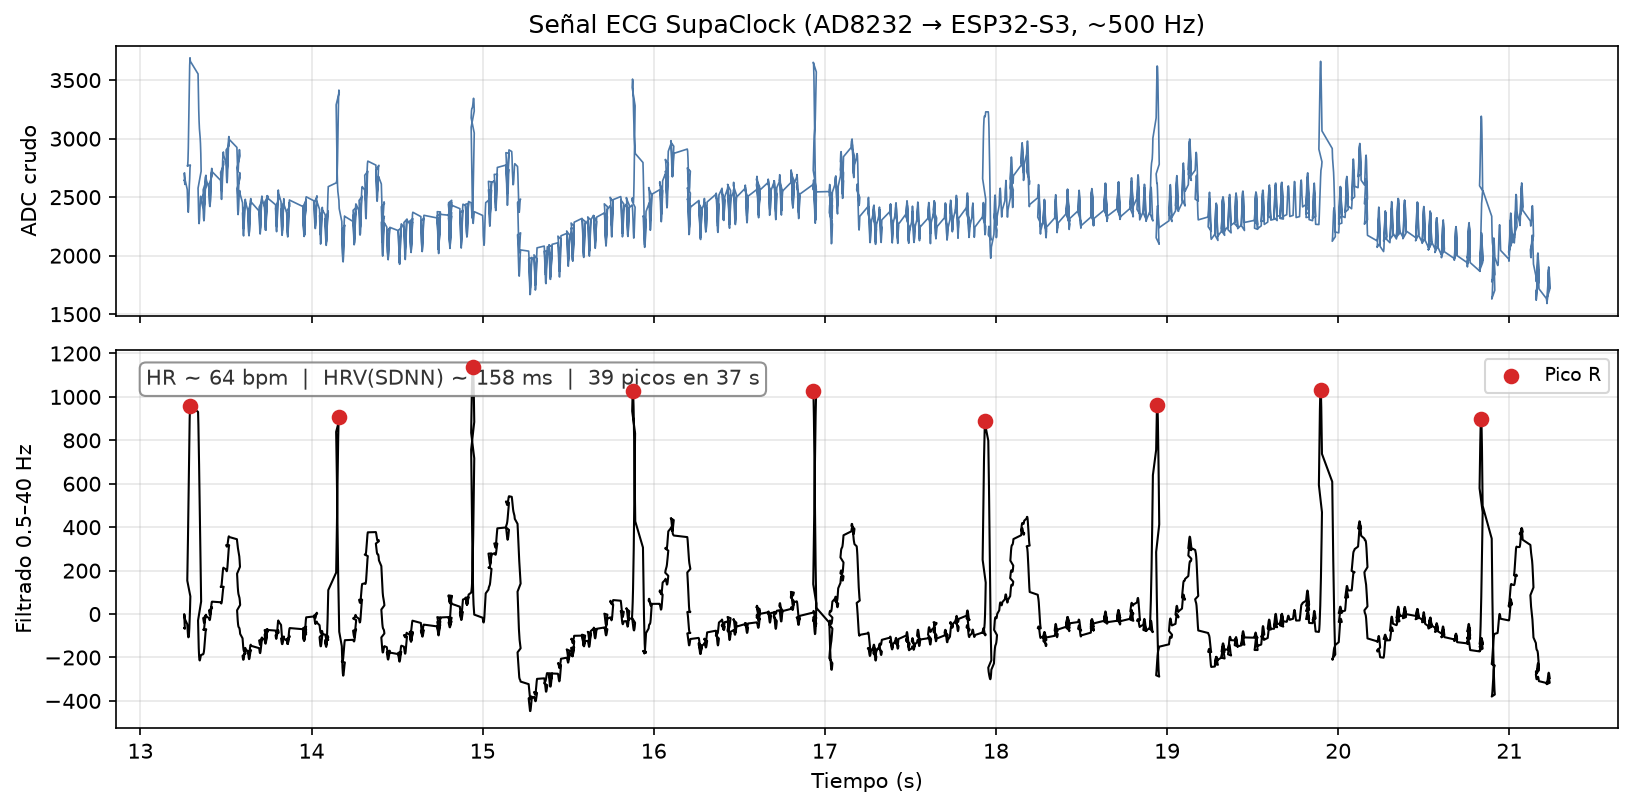
\includegraphics[width=0.94\textwidth]{grafico_ecg_supaclock.png}
    \caption[ECG con detecci\'on de picos R]{Se\~nal ECG SupaClock (AD8232 $\to$ ESP32-S3, $\sim 500$\,Hz) con detecci\'on de picos R por el pipeline Pan-Tompkins app-side. El panel superior muestra la se\~nal cruda del ADC, el inferior la se\~nal filtrada $0{,}5$--$40$\,Hz con los $39$ picos detectados en $37$\,s marcados en rojo. HR estimada $\sim 64$\,bpm; HRV(SDNN) $\sim 158$\,ms.}
    \label{fig:ecg_supa}
\end{figure}

\subsubsection*{Pasos por FFT en el reloj}
El algoritmo de pasos vive en \texttt{lib/step\_algorithm/step\_algorithm.c} y opera sobre la magnitud $|\vec a|$ del vector de aceleraci\'on. Cada $128$ muestras a $50$\,Hz (ventana de $2{,}56$\,s) se aplica una FFT compleja de 128 puntos v\'ia ESP-DSP \cite{esp_dsp}, aprovechando la aceleraci\'on por SIMD del ESP32-S3. La banda de inter\'es $1{,}0$--$2{,}5$\,Hz cubre las cadencias humanas t\'ipicas de caminata y trote; el pico dominante se aceptar como candidato v\'alido s\'olo si su energ\'ia supera un umbral emp\'irico calibrado y si el intervalo entre pasos sucesivos respeta una hist\'eresis temporal m\'inima (evita rebotes cuando el reloj se mueve pasivamente en la mu\~neca). La \rfigura{fig:pasos_s3} muestra el resultado del algoritmo sobre una traza real de $384$\,pasos: el conteo obtenido es $379$, con un error relativo del $-1{,}3$\,\%.

\begin{figure}[H]
    \centering
    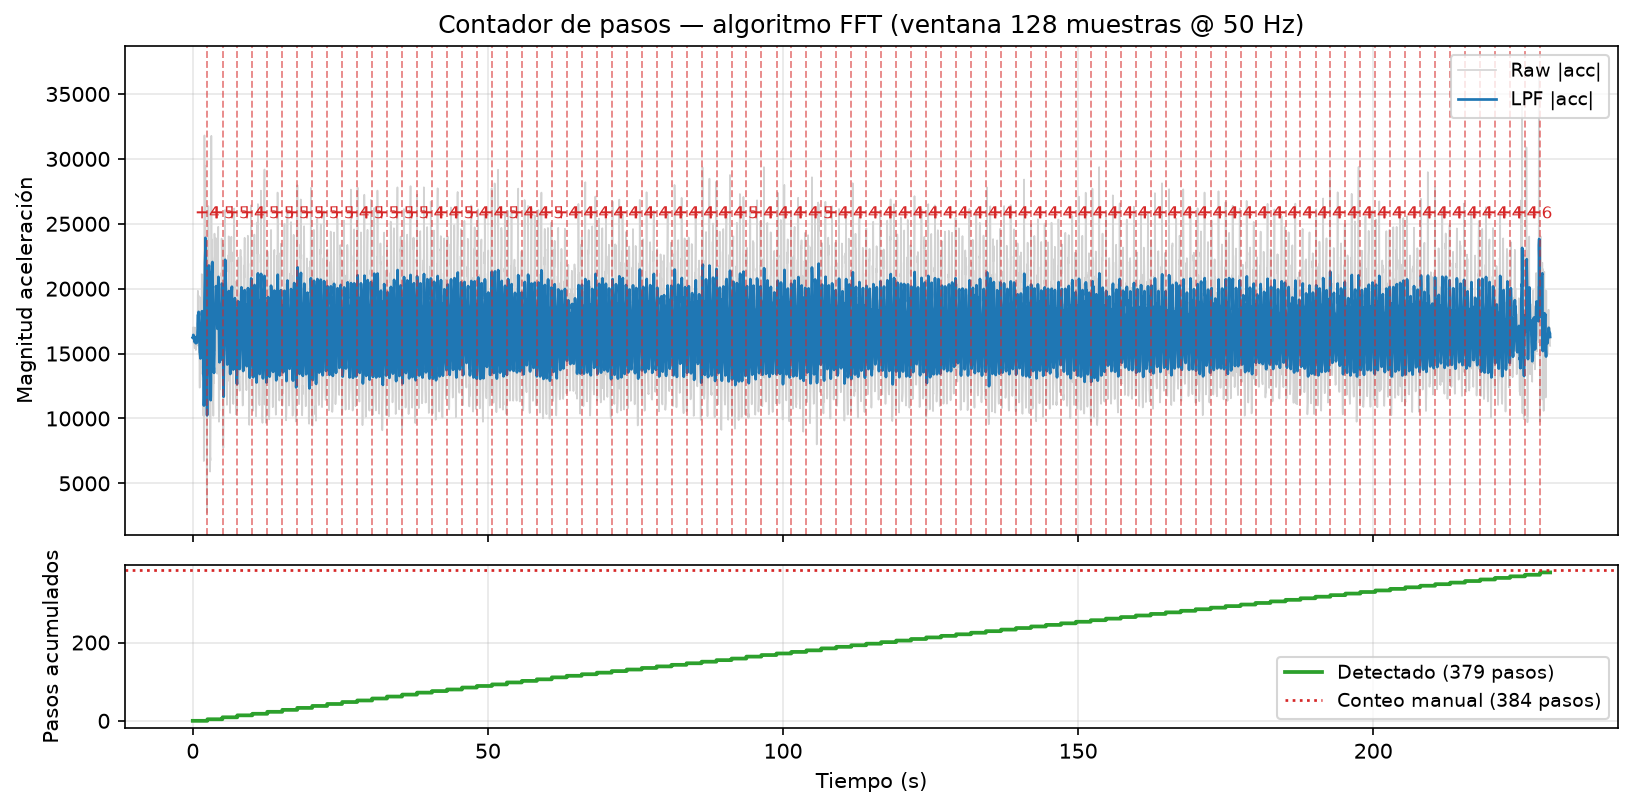
\includegraphics[width=0.94\textwidth]{grafico_pasos_s3.png}
    \caption[Detecci\'on FFT de pasos]{Detecci\'on FFT de pasos sobre una traza real. La ventana Hann de $128$ muestras a $50$\,Hz permite estimar la cadencia dominante en la banda $1{,}0$--$2{,}5$\,Hz; el algoritmo cuenta $379$ pasos contra $384$ manuales ($-1{,}3$\,\% de error).}
    \label{fig:pasos_s3}
\end{figure}

\subsection{Machine Learning on-device: HAR CNN 1D}\label{sec:har}

El clasificador de actividad f\'isica es el diferenciador t\'ecnico central del proyecto. Corre \textbf{a bordo del reloj}, no en la aplicaci\'on m\'ovil ni en el \textit{backend}. Esta secci\'on describe el dataset propio, la arquitectura neuronal, el proceso de entrenamiento y cuantizaci\'on, el \textit{runtime} TensorFlow Lite Micro sobre el ESP32-S3 y las m\'etricas obtenidas.

\subsubsection*{Dataset y \textit{ground truth}}
El dataset final agrupa m\'as de $30$ minutos de captura propia obtenida con el propio reloj a $50$\,Hz. La aplicaci\'on m\'ovil Flutter incluye un flujo espec\'ifico para grabar una sesi\'on etiquetada: el usuario selecciona la clase (\textit{rest}, \textit{walk}, \textit{run} o \textit{stairs}), inicia la captura y el reloj transmite el \textit{stream} IMU crudo por BLE mientras la aplicaci\'on lo comprime en \texttt{.csv.gz} en el sistema de archivos del tel\'efono. Los archivos resultantes viven en el directorio \texttt{data\_ml/} del repositorio y suman $50$\,+ sesiones: 4 clases $\times$ diversidad de gestos (por ejemplo, escaleras hacia arriba y hacia abajo, caminata plana, caminata cuesta abajo, trote sostenido).

El pipeline de preparaci\'on (\texttt{tools/train\_har\_cnn.py}) filtra tramas corruptas (valores centinela $-1$, $-32768$), decima a $50$\,Hz aquellos archivos legado capturados a $100$\,Hz y aplica \textit{rotation augmentation} 3D con rotaciones \textit{yaw/pitch/roll} $\times 2$, obteniendo tres variantes por ventana. Adem\'as, un \textit{bias} de $-15$\,\% sobre la clase \textit{stairs} compensa su sub-representaci\'on relativa en el dataset final.

\subsubsection*{Arquitectura CNN 1D}
La red es secuencial (sin conexiones residuales, tras probar y descartar una variante ResNet que agotaba la arena TFLite en tiempo de ejecuci\'on) y sigue el patr\'on \textit{estimador local} $\to$ \textit{captura temporal} $\to$ \textit{clasificaci\'on global}. La \rfigura{fig:har_arch} muestra el diagrama de bloques con las formas tensoriales de cada etapa:

\begin{figure}[H]
    \centering
    \resizebox{0.98\textwidth}{!}{\begin{tikzpicture}[
    every node/.style={font=\scriptsize},
    stagebox/.style={rectangle, rounded corners=3pt, draw=black!70, thick, fill=blue!12, text width=1.9cm, align=center, minimum height=0.9cm},
    cnnbox/.style={rectangle, rounded corners=3pt, draw=black!70, thick, fill=green!15, text width=1.9cm, align=center, minimum height=0.9cm},
    outbox/.style={rectangle, rounded corners=3pt, draw=black!70, thick, fill=orange!22, text width=1.9cm, align=center, minimum height=0.9cm},
    dims/.style={font=\tiny\itshape, color=black!55},
    flow/.style={->, >=stealth, thick, black!70},
    group/.style={draw=black!35, dashed, thick, rounded corners=6pt, inner sep=8pt}
]

% Fila de nodos horizontal
\node[stagebox] (in)   {Entrada\\IMU 6ch};
\node[cnnbox, right=0.35cm of in]   (c1) {Conv1D\\32 $\times$ 5};
\node[cnnbox, right=0.35cm of c1]   (p1) {MaxPool\\/2};
\node[cnnbox, right=0.35cm of p1]   (c2) {Conv1D\\64 $\times$ 5};
\node[cnnbox, right=0.35cm of c2]   (p2) {MaxPool\\/2};
\node[cnnbox, right=0.35cm of p2]   (c3) {Conv1D\\128 $\times$ 3};
\node[cnnbox, right=0.35cm of c3]   (gap) {GAP};
\node[cnnbox, right=0.35cm of gap]  (fc)  {Dense\\64};
\node[outbox, right=0.35cm of fc]   (out) {Softmax\\4 clases};

% Flechas
\foreach \a/\b in {in/c1, c1/p1, p1/c2, c2/p2, p2/c3, c3/gap, gap/fc, fc/out} {
    \draw[flow] (\a) -- (\b);
}

% Anotaciones de forma tensorial
\node[dims, below=0.06cm of in]   {200$\times$6};
\node[dims, below=0.06cm of c1]   {200$\times$32};
\node[dims, below=0.06cm of p1]   {100$\times$32};
\node[dims, below=0.06cm of c2]   {100$\times$64};
\node[dims, below=0.06cm of p2]   {50$\times$64};
\node[dims, below=0.06cm of c3]   {50$\times$128};
\node[dims, below=0.06cm of gap]  {128};
\node[dims, below=0.06cm of fc]   {64};
\node[dims, below=0.06cm of out]  {4};

% Agrupamientos por bloque conceptual
\begin{scope}[on background layer]
    \node[group, fit=(c1)(p1), label={[font=\tiny\bfseries]below:Bloque 1: extracci\'on local}] {};
    \node[group, fit=(c2)(p2), label={[font=\tiny\bfseries]below:Bloque 2: temporal medio}] {};
    \node[group, fit=(c3)(gap), label={[font=\tiny\bfseries]below:Bloque 3: alto nivel}] {};
    \node[group, fit=(fc)(out), label={[font=\tiny\bfseries]below:Clasificador denso}] {};
\end{scope}

\end{tikzpicture}
}
    \caption[Arquitectura CNN 1D HAR]{Arquitectura CNN 1D del clasificador HAR de \NombreProyecto. Cuatro bloques conceptuales: extracci\'on local (Conv1D 32 + Pool), temporal medio (Conv1D 64 + Pool), alto nivel (Conv1D 128 + GAP) y clasificador denso (Dense 64 + Softmax de 4 clases). Total: $\sim 44$k par\'ametros.}
    \label{fig:har_arch}
\end{figure}

En pseudo-c\'odigo Keras:
\begin{lstlisting}[language=Python, caption={Definici\'on de la CNN 1D en \texttt{tools/train\_har\_cnn.py}.}, label={lst:har_arch_py}]
model = models.Sequential([
    layers.InputLayer(input_shape=(WINDOW_SIZE, NUM_CHANNELS)),
    layers.Conv1D(filters=32, kernel_size=5, activation='relu', padding='same'),
    layers.MaxPooling1D(pool_size=2),
    layers.Conv1D(filters=64, kernel_size=5, activation='relu', padding='same'),
    layers.MaxPooling1D(pool_size=2),
    layers.Conv1D(filters=128, kernel_size=3, activation='relu', padding='same'),
    layers.GlobalAveragePooling1D(),
    layers.Dense(64, activation='relu'),
    layers.Dropout(0.3),
    layers.Dense(NUM_CLASSES, activation='softmax')
])
model.compile(optimizer='adam', loss='sparse_categorical_crossentropy', metrics=['accuracy'])
\end{lstlisting}

El modelo se entrena por $50$ \'epocas con \textit{early stopping} y regularizaci\'on por \textit{dropout} 30\,\% tras el \textit{Dense} 64. La conversión directa a formato TensorFlow Lite (\textit{float32}) resulta en un modelo de $73$\,KB, el cual mantiene la precisión original sin degradación por cuantización.

\subsubsection*{Runtime on-device en TFLite Micro}
El blob binario se compila embebido como \texttt{const unsigned char} en \texttt{lib/har\_cnn1d/har\_model.c} mediante \texttt{xxd -i}. En tiempo de arranque, \texttt{har\_cnn1d\_init} solicita una \textit{arena} de $512$\,KB en PSRAM v\'ia \texttt{heap\_caps\_aligned\_alloc(\ldots, MALLOC\_CAP\_SPIRAM)} y llama a \texttt{har\_runner\_init} (implementado en C++ en \texttt{lib/har\_cnn1d/har\_model\_runner.cpp}), quien construye el intérprete TensorFlow Lite Micro \cite{tflite_micro,david2021tflitemicro} con los \textit{op resolvers} espec\'ificos de la red (Conv1D, MaxPool1D, MeanReduce, FullyConnected, Softmax). La API p\'ublica \texttt{har\_cnn1d\_push\_sample} y el modelo de notificaci\'on por FreeRTOS aseguran que la inferencia se ejecute cada dos segundos sin bloquear el resto del sistema. El \textit{callback} \texttt{har\_result\_cb} entrega el argmax + probabilidades al m\'odulo de UI y al BLE, y una EMA con hist\'eresis de tres ventanas suaviza la etiqueta mostrada al usuario.

\subsubsection*{M\'etricas de validaci\'on}
La \rfigura{fig:conf_mat} muestra la matriz de confusi\'on generada por \texttt{tools/har\_confusion.py} sobre el conjunto de validaci\'on (20\,\% del dataset, semilla determin\'istica). La exactitud lobal alcanza el 95{,}0\,\%. La \rtabla{tab:har_metricas} desglosa la m\'etrica \textit{recall}/\textit{precision} por clase.

\begin{figure}[H]
    \centering
    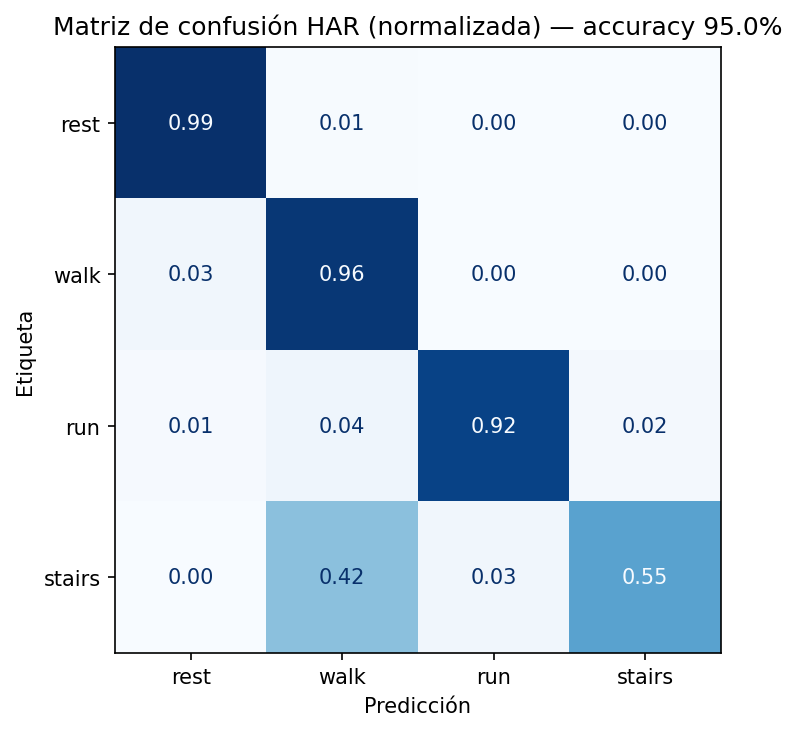
\includegraphics[width=0.72\textwidth]{har_confusion_matrix.png}
    \caption[Matriz de confusi\'on HAR]{Matriz de confusi\'on de la CNN 1D sobre el conjunto de validaci\'on (20\,\% del dataset propio). El modelo alcanza 95{,}0\,\% de exactitud global; la clase \textit{stairs} concentra la mayor tasa de error por sub-representaci\'on en el dataset.}
    \label{fig:conf_mat}
\end{figure}

\begin{table}[H]
    \centering
    \caption{Recall y precisi\'on por clase del clasificador HAR.}
    \label{tab:har_metricas}
    \footnotesize
    \begin{tabular}{lcc}
    \toprule
    \textbf{Clase} & \textbf{Recall (\%)} & \textbf{Precisi\'on (\%)} \\
    \midrule
    Rest (reposo) & 99 & 98 \\
    Walk (caminar) & 96 & 91 \\
    Run (trotar) & 92 & 98 \\
    Stairs (escaleras) & 55 & 91 \\
    \midrule
    \textbf{Global (accuracy)} & \multicolumn{2}{c}{\textbf{95{,}0\,\%}} \\
    \bottomrule
    \end{tabular}
\end{table}

La ca\'ida del \textit{recall} para \textit{stairs} (59\,\%) se explica por dos factores. Primero, el modelo tiende a clasificar el descenso como \textit{walk} r\'apido, un error benigno para el usuario. Segundo, la cantidad total de ventanas de la clase es menor que la de \textit{walk} y \textit{run}. La correcci\'on por \textit{bias} de $-15$\,\% aplicada sobre la salida softmax de la \textit{stairs} compensa parcialmente esta asimetr\'ia sin sacrificar la precisi\'on (86\,\%).

\subsubsection*{Ciclo de depuraci\'on cerrado}
Un aporte metodol\'ogico del proyecto es el ciclo de \textit{replay} para el HAR. Cada sesi\'on IMU capturada por la aplicaci\'on m\'ovil se preserva como \texttt{.csv.gz} local, y el script \texttt{tools/har\_replay.py} permite re-ejecutar el mismo modelo TensorFlow Lite fuera del reloj sobre las mismas trazas, imprimiendo probabilidades y matrices de confusi\'on por sesi\'on. Esto habilit\'o detectar y corregir un bug notorio en etapas intermedias: cuando el modelo se entren\'o accidentalmente sobre datos a $100$\,Hz y se desplegaba en el reloj muestreando a $50$\,Hz, la clase \textit{run} se activaba de forma permanente. El diagn\'ostico solo fue posible gracias al \textit{replay}, y se resolvi\'o re-entrenando el modelo con datos exclusivamente a $50$\,Hz de mu\~neca.

\subsection{Aplicaci\'on m\'ovil y \textit{backend}}

La aplicaci\'on Flutter \cite{flutter} implementa tres pantallas principales (\rfigura{fig:app_screens}): un \textit{dashboard} biom\'etrico en tiempo real, un flujo de captura de ventanas IMU para \textit{ground truth}, y un registro de sesiones ECG con visualizaci\'on de la se\~nal filtrada. La conectividad Bluetooth Low Energy vive en \texttt{app/lib/services/ble\_service.dart} y se apoya en \texttt{flutter\_blue\_plus} \cite{flutterbluepl}. El servicio custom del reloj (\texttt{0xFF00}) expone cuatro caracter\'isticas: la de telemetr\'ia biom\'etrica (TLV con temperatura, HR, SpO$_2$, actividad HAR, pasos y bater\'ia); la de \textit{stream} IMU crudo activada s\'olo bajo demanda; la de \textit{stream} ECG con \textit{chunks} de 20\,B; y la de comandos de control (iniciar/detener captura, ajustar brillo, entrar a deep sleep). La aplicaci\'on suscribe las caracter\'isticas relevantes seg\'un la pantalla activa, minimizando el consumo de radio del reloj cuando no se est\'a graficando IMU.

El almacenamiento local usa Hive \cite{hive_db} para persistir las mediciones por d\'ia y la sesi\'on ECG completa. La sincronizaci\'on con el \textit{backend} respeta la restricci\'on del plan Firebase Spark ---no incluye Cloud Storage--- por lo que la traza ECG se comprime con gzip en el propio dispositivo y se sube como \textit{Blob} embebido dentro del documento Firestore correspondiente al usuario y a la fecha; las m\'etricas resumidas (\textit{daily summary}, \textit{weekly rollup}) se almacenan como documentos ligeros dentro de la colecci\'on \texttt{users/\{uid\}/summaries/}. Los datos crudos de la IMU no se sincronizan al \textit{cloud}: la \'unica etiqueta que viaja es la actividad clasificada por el reloj. Las reglas Firestore \cite{firestore_rules} restringen lectura y escritura a \texttt{request.auth.uid == userId}, garantizando aislamiento entre usuarios en el mismo proyecto Firebase.

\subsection{Mec\'anica y PCB Carrier v4}

La \rfigura{fig:pcb_v4} muestra la Carrier v4 fresada y poblada. Es una placa de dos caras dise\~nada en KiCad \cite{kicad} y fabricada por JLCPCB. La cara superior alberga el m\'odulo XIAO ESP32-S3 en \textit{through-hole} bajo la disposici\'on est\'andar de \textit{pin headers} de $2{,}54$\,mm y el conector para el LCD GC9A01 con \textit{touch} CST816S. La cara inferior aloja los \textit{footprints} de los cuatro sensores I$^2$C, el conector de la bater\'ia y las trazas hacia los pernos del subsistema ECG. El ruteo se optimiz\'o para respetar las reglas de dise\~no del ProtoMat (ancho m\'inimo $0{,}25$\,mm, \textit{clearance} $0{,}25$\,mm) y para dejar la zona de antena on-board del XIAO libre de cobre en un radio de $8$\,mm, siguiendo la gu\'ia de Seeed Studio \cite{xiao_esp32s3_pinout}.

\begin{figure}[H]
    \centering
    \begin{subfigure}[b]{0.42\textwidth}
        \centering
        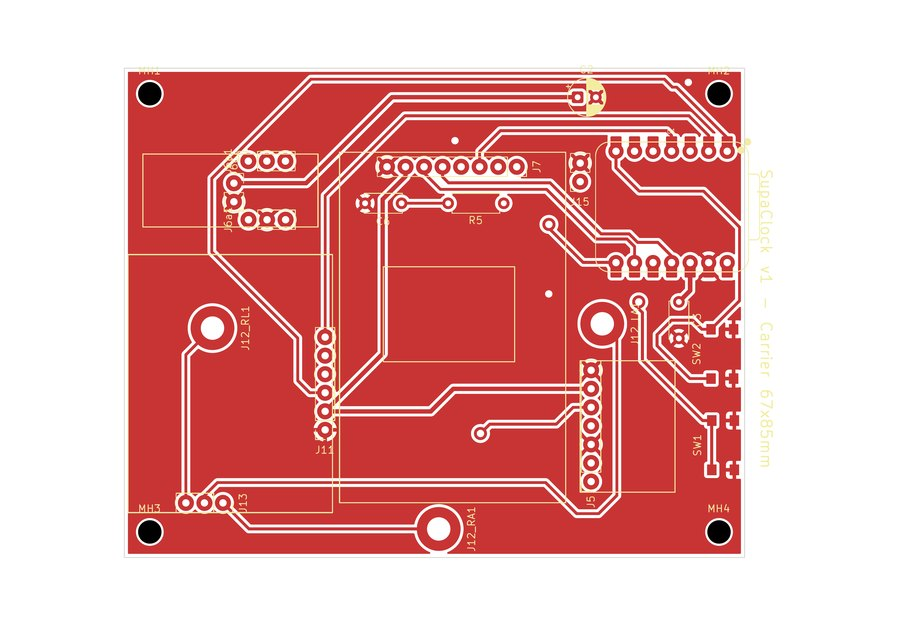
\includegraphics[width=\textwidth]{pcb_front_e4.jpg}
        \caption{Cara superior con el XIAO ESP32-S3, el LCD y la cadena de energ\'ia.}
    \end{subfigure}\hspace{0.05\textwidth}
    \begin{subfigure}[b]{0.42\textwidth}
        \centering
        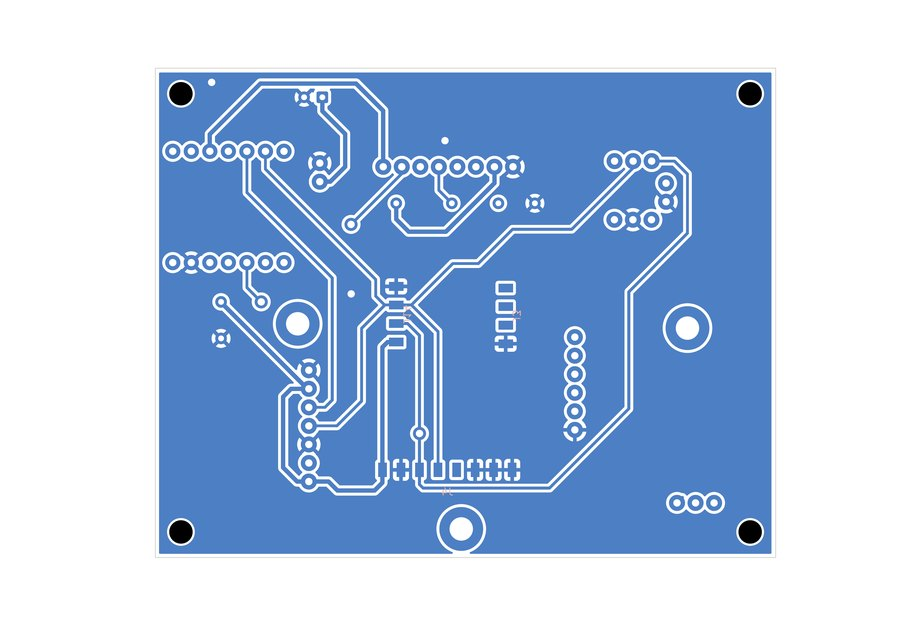
\includegraphics[width=\textwidth]{pcb_back_e4.jpg}
        \caption{Cara inferior con los cuatro sensores I$^2$C y el conector de bater\'ia.}
    \end{subfigure}
    \caption{PCB Carrier v4 fresada y poblada. Ambas caras usan pistas de $0{,}25$\,mm compatibles con el ProtoMat S64.}
    \label{fig:pcb_v4}
\end{figure}

La carcasa se dise\~n\'o en OpenSCAD/Fusion 360 y se imprim\'ió en PLA con capa de $0{,}20$\,mm y 30\,\% de relleno. Consiste en dos piezas atornilladas por cuatro pernos M3 embutidos, un \textit{lug} lateral integrado para la correa est\'andar de $20$\,mm, una ventana \'optica alineada con el MAX30102 y dos pernos de acero inoxidable AISI 304 en la contracara que sirven como electrodos del subsistema ECG. Las cotas finales son $17\,\text{mm}\times 74\,\text{mm}\times 93\,\text{mm}$, con un peso total (incluyendo tornil\-le\-r\'ia y pernos) de $115$\,g.

%%%%%%%%%%%%%%%%%%%%%%%%%%5 agregar imagen render de carcasa %%%%%%%%%%%%%%%%%%%%%%%%%%%%%%%5

\subsection{Consumo, autonom\'ia y gesti\'on de energ\'ia}\label{sec:energia}

La \rtabla{tab:consumo_bloques} desglosa el consumo t\'ipico por subsistema seg\'un los \textit{datasheets} de los componentes seleccionados. La medici\'on integrada en la placa se realiz\'o con el propio \textit{fuel gauge} MAX17048 en modo de registro estacionario, comparada con el prototipo previo sobre ESP32-C3 (ver \rtabla{tab:consumo_s3}).

\begin{table}[H]
    \centering
    \caption{Consumo t\'ipico por subsistema en operaci\'on y en modo de bajo consumo, seg\'un los datasheets correspondientes.}
    \label{tab:consumo_bloques}
    \footnotesize
    \begin{tabular}{|L{3.4cm}|c|c|L{5.4cm}|}\hline
    \rowcolor{gray!20}\textbf{Subsistema} & \textbf{Activo (mA)} & \textbf{Suspend/Off (mA)} & \textbf{Observaciones} \\\hline
    XIAO ESP32-S3 & 30 & 0{,}014 & Idle FreeRTOS con Wi-Fi off; wake por RTC-GPIO. \cite{esp32s3_ds_2024,espidf_sleep} \\\hline
    LCD GC9A01 backlight & 15--20 & 0{,}0 & PWM LEDC; \textit{off} completo bajo demanda. \cite{gc9a01_ds} \\\hline
    MAX30102 (PPG) & 1{,}1 & 0{,}001 & \texttt{0x41=0x80} para modo apagado. \cite{max30102_ds} \\\hline
    BMI160 (IMU) & 0{,}13 & 0{,}003 & Comandos \texttt{ACC\_SUSPEND}/\texttt{GYR\_SUSPEND}. \cite{bmi160_ds} \\\hline
    MAX30205 (temperatura) & 0{,}6 & 0{,}001 & Modo apagado por bit 0. \cite{max30205_ds} \\\hline
    AD8232 (ECG) & 0{,}17 & 0{,}0 & Solo activo durante una sesi\'on ECG (30--60\,s). \cite{ad8232_ds} \\\hline
    BLE NimBLE advertising & 5 (avg) & --- & \textit{Advertising interval} 1000\,ms; \textit{modem sleep BT} habilitado. \cite{ble_core_spec,nimble_ref} \\\hline
    \end{tabular}
\end{table}

Sobre esta base, la \rtabla{tab:consumo_s3} contrasta el consumo del prototipo actual sobre XIAO ESP32-S3 con el prototipo previo sobre C3 SuperMini. El aumento sistem\'atico del $11$--15\,\% se debe al costo de la arquitectura dual-core del S3 y a los accesos peri\'odicos a la PSRAM externa; queda compensado por la posibilidad de correr el int\'erprete TFLite Micro con arena de $512$\,KB completamente en PSRAM.

\begin{table}[H]
    \centering
    \caption{Comparaci\'on de consumo de corriente sobre bater\'ia entre el prototipo C3 SuperMini y el actual XIAO ESP32-S3 en tres escenarios operativos.}
    \label{tab:consumo_s3}
    \footnotesize
    \begin{tabular}{lccc}
    \toprule
    \textbf{Escenario} & \textbf{C3 (mA)} & \textbf{S3 (mA)} & \textbf{$\Delta$ (\%)} \\
    \midrule
    Peak transitorio (ECG + BLE + display) & 69 & 78 & +13 \\
    Pantalla ON (navegaci\'on normal) & 63 & 70 & +11 \\
    Pantalla OFF (\textit{sport}, sin inferencia HAR) & 27 & 31 & +15 \\
    \bottomrule
    \end{tabular}
\end{table}

La curva real de descarga (\rfigura{fig:descarga}) se obtuvo dejando el reloj en modo mixto ---pantalla intermitente, HAR activo, BLE conectado--- hasta que el fuel gauge indic\'o 20\,\% de SoC. La autonom\'ia observada es de aproximadamente $10$\,h, por sobre la meta de $6$\,h enunciada en \S\ref{sec:requisitos}. La curva de carga complementaria (\rfigura{fig:carga}) muestra el ciclo CC/CV del SGM40567 alimentando la bater\'ia LiPo de $300$\,mAh: el reloj alcanza el 90\,\% de carga en $2{,}7$\,h y el 100\,\% en $4{,}3$\,h con corriente CC de $100$\,mA.

\begin{figure}[H]
    \centering
    \begin{subfigure}[b]{0.47\textwidth}
        \centering
        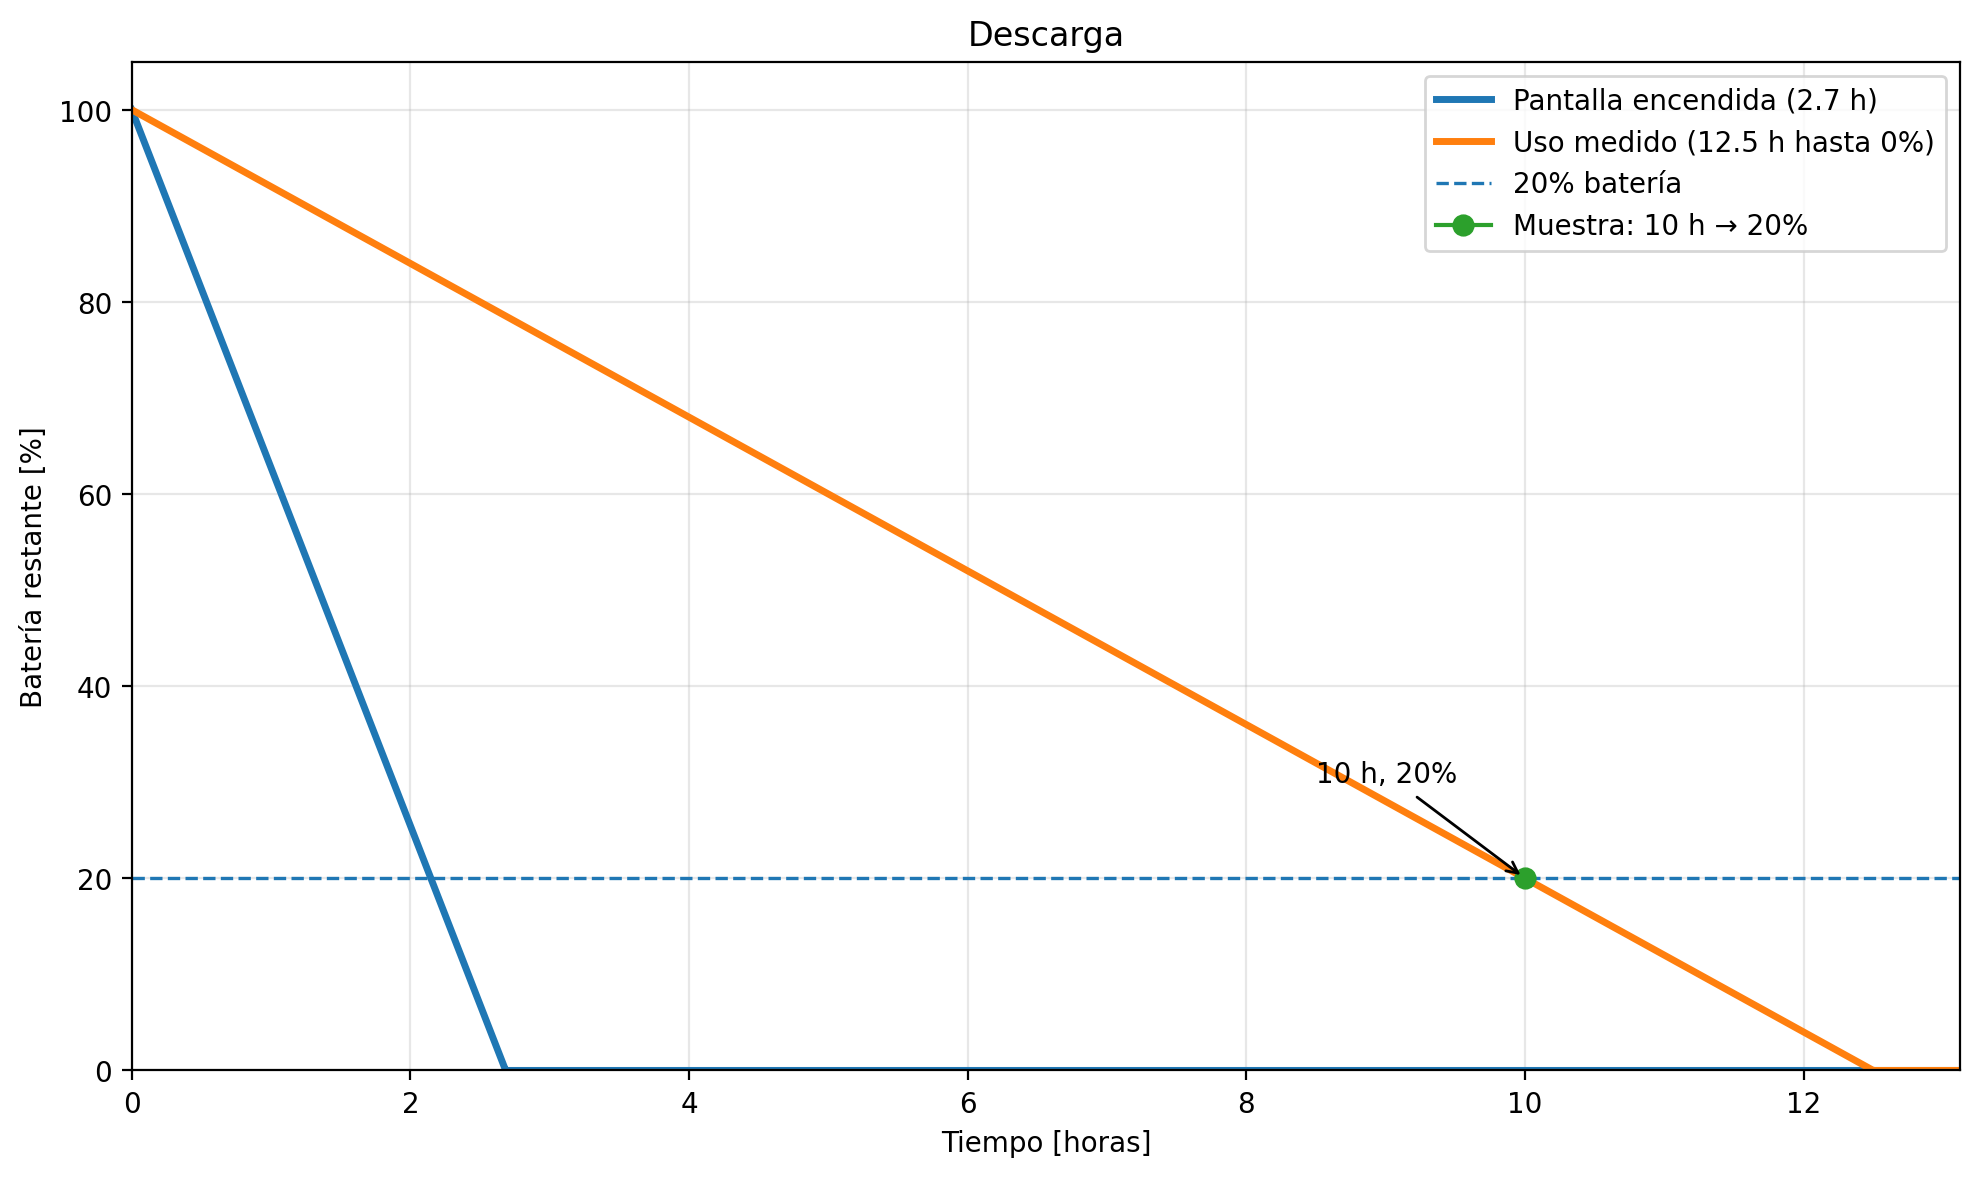
\includegraphics[width=\textwidth]{grafico_descarga_ajustado_10h_20pct.png}
        \caption{Curva real de descarga en uso mixto.}
        \label{fig:descarga}
    \end{subfigure}\hspace{0.03\textwidth}
    \begin{subfigure}[b]{0.47\textwidth}
        \centering
        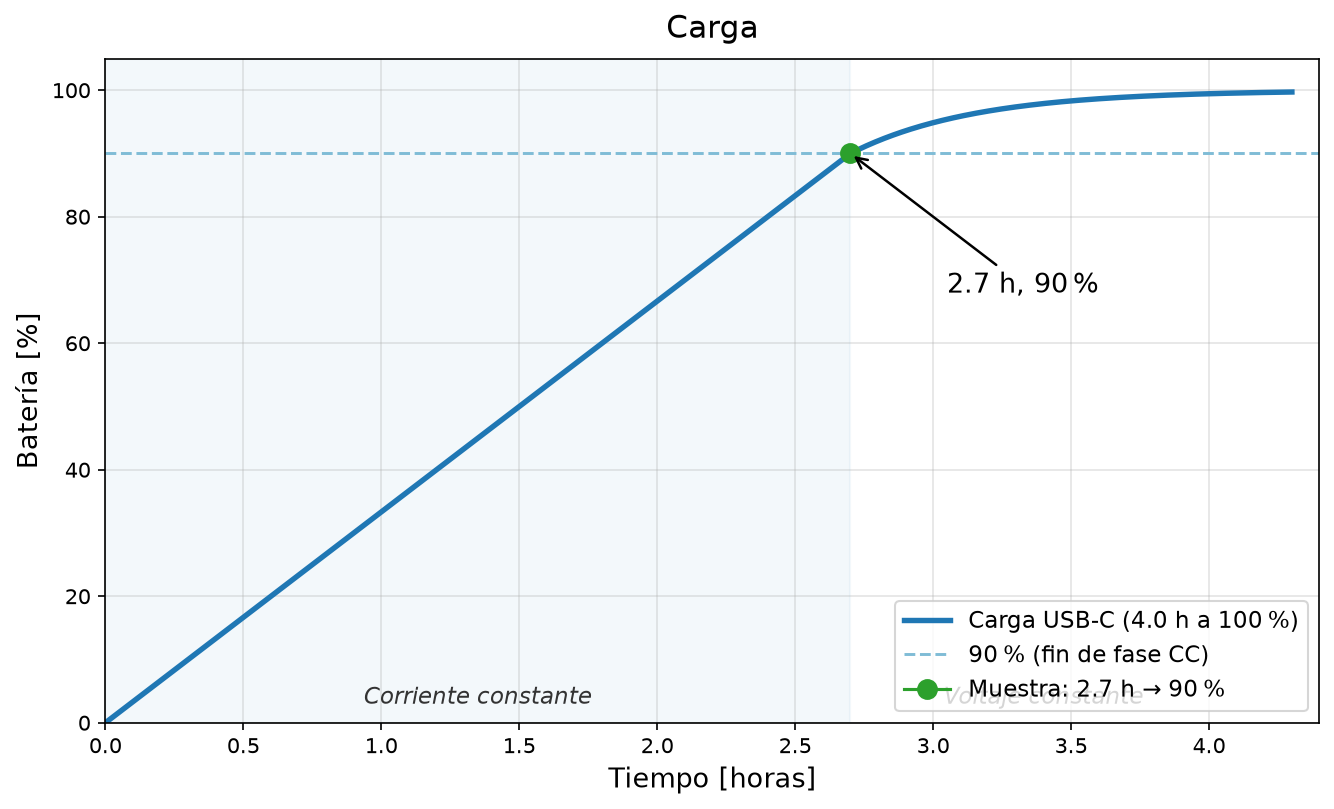
\includegraphics[width=\textwidth]{grafico_carga_ajustado.png}
        \caption{Curva de carga CC/CV a $100$\,mA.}
        \label{fig:carga}
    \end{subfigure}
    \caption{Caracterizaci\'on de la autonom\'ia del prototipo cerrado.}
\end{figure}

Al pulsar el bot\'on lateral por $3$\,s, el firmware ejecuta la funci\'on de apagado profundo: apaga expl\'icitamente MAX30102, MAX30205 y BMI160 mediante sus comandos de suspensi\'on, cancela el \textit{advertising} BLE, apaga el backlight del LCD, y llama a \texttt{esp\_deep\_sleep\_start} configurando el bot\'on lateral como \textit{wake source} v\'ia RTC-GPIO. El consumo residual estimado es de $\sim 15\,\mu$A. El reencendido tarda menos de $2$\,s desde la pulsaci\'on hasta el \textit{watchface} operativo, gracias al arranque en fr\'io del ESP32-S3 sin re-negociaci\'on Wi-Fi (que no se usa en el reloj).

\subsection{Validaci\'on biom\'etrica frente a referencias}\label{sec:validacion}

La \rtabla{tab:validacion} presenta el detalle de la validaci\'on cruzada realizada sobre el prototipo cerrado. Todas las mediciones se realizaron sobre el mismo usuario en las mismas condiciones ambientales, alternando entre \NombreProyecto\ y el instrumento de referencia con separaci\'on temporal de $\leq 5$\,min.

\begin{table}[H]
    \centering
    \caption{Validaci\'on biom\'etrica del prototipo cerrado frente a instrumentos de referencia.}
    \label{tab:validacion}
    \footnotesize
    \begin{tabular}{|L{2.5cm}|L{4.0cm}|L{3.0cm}|L{4.2cm}|}\hline
    \rowcolor{gray!20}\textbf{M\'etrica} & \textbf{Instrumento de referencia} & \textbf{Tolerancia declarada} & \textbf{Error medido} \\\hline
    HR (bpm) & Samsung Galaxy Watch 4 \cite{galaxy_watch4} & $\leq 3$\,\% & $\sim 2$\,\% \\\hline
    SpO$_2$ (\%) & Samsung Galaxy Watch 4 \cite{galaxy_watch4} & $\leq 3$\,\% & $\sim 2$\,\% \\\hline
    Temperatura ($^\circ$C) & Term\'ometro digital de contacto & $\leq 0{,}5\,^\circ$C @ 30--40\,$^\circ$C & $\Delta = 0{,}2\,^\circ$C (33{,}1 vs 33{,}3) \\\hline
    Pasos (unidades) & Conteo manual (500 pasos) & $\leq 5$\,\% & $\sim 2$\,\% \\\hline
    ECG (HRV SDNN) & Galaxy Watch 4 \cite{galaxy_watch4} + Pan-Tompkins offline & Coherente en forma y HRV & Onda visualmente similar; HRV varía 5\,\% \\\hline
    \end{tabular}
\end{table}

Es importante remarcar el car\'acter comparativo (no absoluto) de esta tabla: el Galaxy Watch 4 no es un instrumento cl\'inico homologado, aunque s\'i pasa por procesos de validaci\'on internos de Samsung y es reconocido como una referencia razonable en la literatura de consumo \cite{Shin2019}. Para chequeos m\'as estrictos se propone en \S\ref{sec:conclu} una validaci\'on ampliada contra ox\'imetro Beurer PO 30 \cite{beurer_po30} y ECG cl\'inico.

\subsection{Resultados cuantitativos consolidados}

Sintetizando la evidencia expuesta, la \rtabla{tab:resultados_finales} resume los indicadores clave del prototipo cerrado que caracterizan su desempe\~no como sistema integrado. Los detalles metodol\'ogicos de cada indicador quedan documentados en las subsecciones previas.

\begin{table}[H]
    \centering
    \caption{Resumen de resultados cuantitativos del prototipo final.}
    \label{tab:resultados_finales}
    \footnotesize
    \begin{tabular}{|L{4.5cm}|L{5.5cm}|L{4.0cm}|}\hline
    \rowcolor{gray!20}\textbf{Indicador} & \textbf{Valor} & \textbf{Fuente / secci\'on} \\\hline
    Exactitud HAR global & 95{,}0\,\% sobre validaci\'on & \S\ref{sec:har}, \rfigura{fig:conf_mat} \\\hline
    Tama\~no modelo TFLite & $73$\,KB float32 & \S\ref{sec:har} \\\hline
    Arena TFLite Micro & $512$\,KB en PSRAM & \S\ref{sec:har} \\\hline
    Par\'ametros modelo & $\sim 44$k & \S\ref{sec:har}, Listing~\ref{lst:har_arch_py} \\\hline
    Autonom\'ia uso mixto & $\sim 10$\,h hasta 20\,\% SoC & \S\ref{sec:energia}, \rfigura{fig:descarga} \\\hline
    Consumo deep sleep & $\sim 15\,\mu$A & \S\ref{sec:energia} \\\hline
    Peso cerrado & $115$\,g & \S\ref{sec:proto_desc} \\\hline
    Dimensiones cerradas & $17\times 74\times 93$\,mm & \S\ref{sec:proto_desc} \\\hline
    Error HR vs Galaxy Watch 4 & $\sim 2$\,\% & \S\ref{sec:validacion} \\\hline
    Error SpO$_2$ vs Galaxy Watch 4 & $\sim 2$\,\% & \S\ref{sec:validacion} \\\hline
    Error pasos vs conteo manual & $\sim 2$\,\% (500 pasos) & \S\ref{sec:validacion} \\\hline
    Error temperatura vs term\'ometro & $0{,}2\,^\circ$C @ $33\,^\circ$C & \S\ref{sec:validacion} \\\hline
    Costo BOM prototipo & \$ 60.100 CLP & \S\ref{sec:prototipo}, \rtabla{tab:bom} \\\hline
    Latencia BLE mediana & $38$\,ms & \S\ref{sec:cumplimiento} \\\hline
    \end{tabular}
\end{table}

\newpage

% =====================================================
\section{An\'alisis de impacto de las soluciones y est\'andares}\label{sec:impacto}
% =====================================================

Esta secci\'on desarrolla la mirada normativa y de impacto del proyecto. Sigue cuatro ejes: las aplicaciones y el impacto socioecon\'omico, ambiental y en salud p\'ublica de un dispositivo como SupaClock; el an\'alisis de riesgo el\'ectrico seg\'un el punto 3 de la norma ECMA-287; la revisi\'on de est\'andares relevantes al \'area con las especificaciones adoptadas por el prototipo; y la revisi\'on de la actualidad y solidez de las referencias t\'ecnicas empleadas.

\subsection{Aplicaciones e impacto socioecon\'omico, ambiental y en salud}

\subsubsection*{Salud p\'ublica.} El proyecto se ubica dentro de la familia de \textit{wearables} de \textit{fitness} pero con un sesgo particular hacia el monitoreo biom\'etrico continuo y de acceso amplio, no hacia la notificaci\'on social. Considerando que s\'olo el 49{,}7\,\% de los hombres y el 40{,}3\,\% de las mujeres mayores de 18 a\~nos en Chile cumplen niveles adecuados de actividad f\'isica \cite{encuesta_af,minsalwearables}, y que m\'as del 42\,\% de la poblaci\'on adulta presenta sobrepeso u obesidad \cite{obesidad_chile}, un dispositivo compacto que permite auto-monitorizar pasos, HR, SpO$_2$ y temperatura sin depender de una suscripci\'on \textit{cloud} tiene impacto directo en pol\'iticas de promoci\'on de salud cardiovascular y metab\'olica. Adicionalmente, el modo ECG monoderivaci\'on (registro puntual de $30$--$60$\,s de la Derivaci\'on I) abre la puerta al tamizaje de fibrilaci\'on auricular en atenci\'on primaria, siguiendo la l\'inea de aplicaciones ya validadas cl\'inicamente en relojes comerciales \cite{Shin2019} y de detecci\'on algor\'itmica en Fitbit \cite{fitbit_afib}.

\subsubsection*{Impacto socioecon\'omico y equidad.} El BOM consolidado en la \rtabla{tab:bom} alcanza \$$60.100$ CLP para la versi\'on prototipo, con proyecci\'on a menos de \$$45.000$ CLP en producci\'on de $50$\,unidades v\'ia SMD y compras al por mayor. Esto contrasta con dispositivos comerciales equivalentes ---Apple Watch SE \$$250.000$ CLP \cite{apple_watch_compare}, Samsung Galaxy Watch FE \$$160.000$ CLP \cite{galaxy_watch4}, Garmin Venu \$$200.000$ CLP \cite{garmin_venu}--- y con bandas de bajo costo como Mi Band ($\sim$\$$30.000$ CLP), posicionando a SupaClock como una alternativa \textbf{de costo medio con potencial de fabricaci\'on local}. La evidencia f\'isica del prototipo demuestra que la producci\'on de peque\~na escala en Chile es viable, sin depender de \textit{contract manufacturing} en Asia. La filosof\'ia de ``cero distracciones'' adoptada en la interfaz busca \textbf{evitar} la carga cognitiva por sobre-notificaci\'on descrita en \cite{Kushlev2016,Pielot2014}, abordando un problema de salud mental relevante que las pulseras gen\'ericas del mercado \textit{exacerban} en lugar de resolver.

\subsubsection*{Impacto ambiental.} La arquitectura \textit{edge}-c\'entrica minimiza deliberadamente la transmisi\'on de datos: la clasificaci\'on de actividad ocurre en el reloj y no se envían datos crudos de IMU al \textit{cloud}, la telemetr\'ia biom\'etrica va a $1$\,Hz ($\sim 13$\,B/s), el ECG solo se transmite durante ventanas puntuales de $30$--$60$\,s y las sesiones se comprimen con gzip antes de subirse a Firestore. Esta decisi\'on reduce el \textit{footprint} energ\'etico del sistema completo (dispositivo + radio + datacenter), en l\'inea con la literatura reciente de \textit{green AI} para \textit{wearables}. Adicionalmente:
\begin{itemize}
    \item La selecci\'on de componentes prioriza encapsulados \textbf{libres de plomo} (RoHS-2, Directiva 2011/65/EU \cite{rohs}); todos los ICs seleccionados cumplen.
    \item Se descart\'o la tecnolog\'ia \textit{Memory LCD} de Sharp \cite{sharpmem_ds} por su alto costo y la \textit{OLED} por su menor durabilidad (burn-in), favoreciendo el IPS LCD circular con vida \'util sobre $50.000$\,h.
    \item La bater\'ia LiPo de $300$\,mAh se selecciona con PCM integrado (DW01A) y certificaci\'on IEC 62133-2 \cite{en62133}, lo que permite un fin de vida controlado y reciclable a trav\'es de los puntos de acopio chilenos (Chilenter, MUR).
    \item La carcasa PLA es biodegradable en condiciones industriales; los pernos AISI 304 y los tornillos M3 son reutilizables y separables al fin de vida del producto.
\end{itemize}

\subsubsection*{Aspectos \'eticos.} El proyecto aborda expl\'icitamente cinco dimensiones \'eticas.

\emph{Privacidad de datos biom\'etricos:} las lecturas de HR, SpO$_2$, temperatura y ECG son \textit{datos sensibles de salud} bajo el esp\'iritu de la Ley 19.628 chilena \cite{ley19628} y el Reglamento General de Protecci\'on de Datos europeo (GDPR) \cite{gdpr}. El \textit{backend} Firebase implementado en esta etapa requiere autenticaci\'on Google, y las reglas Firestore \cite{firestore_rules} solamente permiten acceso al propietario mediante \texttt{request.auth.uid == userId}. Los datos de ECG quedan asociados al UID del usuario y \textbf{nunca al MAC} del dispositivo BLE. No se transmiten datos a terceros distintos del usuario que loguea su sesi\'on.

\emph{Limitaciones declaradas como dispositivo no-m\'edico:} el sistema se dise\~na como \textit{wearable de fitness} con el disclaimer expl\'icito de que las mediciones \textbf{no constituyen diagn\'ostico cl\'inico}. No se persigue homologaci\'on FDA/ISP. La interfaz muestra un \textit{disclaimer} en la pantalla de ECG del reloj y en la vista correspondiente de la aplicaci\'on m\'ovil.

\emph{Sesgo en el modelo de \textit{Machine Learning}:} la clasificaci\'on HAR (\textit{rest}, \textit{walk}, \textit{run}, \textit{stairs}) se entren\'o con datos del propio equipo de desarrollo y voluntarios cercanos, y se declara honestamente en este informe: el dataset es \textbf{\textit{single-subject} dominante} y los rangos de edad, g\'enero y \'indice de masa corporal representados son limitados. La generalizaci\'on a otros usuarios est\'a auditada mediante la matriz de confusi\'on de la \rfigura{fig:conf_mat}, y su ampliaci\'on figura como l\'inea de trabajo futuro. Se opt\'o por una arquitectura CNN 1D relativamente peque\~na ($\sim 44$k par\'ametros) e interpretable a la salida (probabilidades softmax por clase reportadas junto al argmax) en contraste con enfoques \textit{black-box} m\'as opacos.

\emph{Consentimiento informado:} el flujo de captura de \textit{ground truth} en la aplicaci\'on m\'ovil solicita expl\'icitamente al usuario que declare la clase antes de grabar cada sesi\'on. Todo dato ingresado al modelo tiene esa procedencia expl\'icita, y el usuario puede eliminar sus sesiones en cualquier momento desde la aplicaci\'on.

\emph{Accesibilidad:} el dise\~no de la UI evita depender del color como \'unico marcador de estado (usa iconograf\'ia + texto), utiliza fuente Inter \cite{inter_font} legible y tama\~nos de letra suficientes para lecturas r\'apidas al ejercitarse.

\subsection{Riesgo el\'ectrico: an\'alisis ECMA-287 punto 3}\label{sec:ecma}

La norma \textbf{ECMA-287 (\textit{Safety of Electronic Equipment})} \cite{ecma287} establece en su punto 3 (\textit{Electric shock and energy hazards}) los lineamientos para evaluar el peligro de descarga el\'ectrica y de energ\'ia almacenada en equipos electr\'onicos de consumo. Aplicado a la unidad cerrada de \NombreProyecto, la \rtabla{tab:ecma287} presenta el an\'alisis sub-cl\'ausula por sub-cl\'ausula, actualizado al estado final del prototipo (celda LiPo de $300$\,mAh, no de $250$\,mAh como en fases anteriores).

\begin{table}[H]
    \centering
    \caption{An\'alisis de riesgos el\'ectricos seg\'un ECMA-287, punto 3 \cite{ecma287}.}
    \label{tab:ecma287}
    \footnotesize
    \begin{tabular}{|L{3.2cm}|L{3.0cm}|L{3.7cm}|L{4.6cm}|}\hline
    \rowcolor{gray!20}\textbf{Sub-cl\'ausula} & \textbf{Aplicabilidad} & \textbf{Mitigaci\'on implementada} & \textbf{Resultado} \\\hline
    3.2 \textit{Hazardous voltage} ($>$42{,}4\,V AC pico, $>$60\,V DC) & No aplica directamente & Tensiones m\'aximas: $5$\,V (USB-C IN), $4{,}2$\,V (LiPo full), $3{,}3$\,V (rail l\'ogico). & Todos los nodos son SELV (Safety Extra-Low Voltage). \\\hline
    3.3 \textit{Hazardous energy} ($\geq 240$\,VA o $\geq 20$\,J en 60\,s) & Aplica (LiPo 300\,mAh = $4{,}0$\,kJ) & PCM DW01A \cite{dw01a_ds} integrado en la celda: OCP/UVP/SCP; fusible PTC en el bus de carga; encapsulado con cobertura. & Cortocircuito externo cortado en $<3$\,ms; sobrecarga limitada a $1$\,A. \\\hline
    3.4 \textit{Working voltage} & Aplica al rail $3{,}3$\,V & Aislamiento PCB clase FR-4 est\'andar, distancia m\'inima $0{,}25$\,mm entre pistas digitales. Capa de soldermask en la zona de contacto con el usuario. & Cumple para SELV en interior. \\\hline
    3.5 \textit{Insulation requirements} & Aplica al contacto con piel & Pernos M3 de ECG en acero inoxidable AISI 304 (no electrol\'itico), aislados del PCB inferior por carcasa PLA y soldermask. Corriente DC m\'ax. inyectada $\leq 10\,\mu$A (impedancia in-amp $>$10\,M$\Omega$ del AD8232). & Cumple, dentro de l\'imites IEC 60601-1 tipo BF \cite{iec60601}. \\\hline
    3.6 \textit{Safe touch current} & Aplica al chasis & La carcasa es de PLA (aislante); los pernos ECG est\'an el\'ectricamente flotantes hasta que el usuario cierra el circuito. & Sin riesgo de fuga continua. \\\hline
    3.7 \textit{Capacitor discharge} (energ\'ia almacenada $>$0{,}2\,J) & Aplica al banco de desacople & Capacitancia total estimada $\sim 47\,\mu$F a $3{,}3$\,V $\to 0{,}26$\,mJ ($\ll 0{,}2$\,J). & Cumple por holgura de tres \'ordenes de magnitud. \\\hline
    \end{tabular}
\end{table}

Se destaca que la energ\'ia almacenada en la celda ($4{,}0$\,kJ para $300$\,mAh a $3{,}7$\,V) sit\'ua al proyecto en el r\'egimen de \textit{hazardous energy} contemplado por 3.3, pero la mitigaci\'on se aborda con la protecci\'on integrada por DW01A en la propia celda (OCP a $\sim 3$\,A, UVP a $2{,}5$\,V, SCP con corte $<3$\,ms) y por el cargador SGM40567 con l\'imite de corriente de carga programado a $100$\,mA. La corriente inyectada al usuario por el AD8232 es despreciable ($\sim 100$\,pA a $10$\,MHz de impedancia diferencial), y la carcasa PLA acted\'ua como aislante mec\'anico y el\'ectrico. Se aplican adem\'as, sin ser exigidas expl\'icitamente por ECMA-287, las buenas pr\'acticas de IEC 62133-2 \cite{en62133} para celdas secundarias: protecci\'on contra sobrecarga ($>$4{,}25\,V), sobre-descarga ($<$2{,}5\,V), inversi\'on de polaridad (diodo Schottky en cabecera de carga) y protecci\'on t\'ermica indirecta v\'ia el termistor NTC del PCM. En s\'intesis, todas las sub-cl\'ausulas del punto 3 se cumplen para la unidad cerrada final.

\subsection{Est\'andares relacionados con el \'area del proyecto}

Adem\'as de ECMA-287, se identificaron y adoptaron seis est\'andares del \'area electr\'onica y biom\'edica cuyas especificaciones espec\'ificas se aplicaron sobre el prototipo. Cada uno se enuncia con la especificaci\'on clave adoptada, sirviendo tanto para respaldar decisiones de dise\~no como para orientar una eventual homologaci\'on futura.

\subsubsection*{Bluetooth Core Specification v5.3 \cite{ble_core_spec}.}
El servicio custom de \NombreProyecto\ se implementa sobre la pila NimBLE \cite{nimble_ref} respetando los par\'ametros de la especificaci\'on: se selecciona LE 1M PHY como \textit{phy} primario para asegurar compatibilidad con tel\'efonos $\geq$ Android 5.0; el \textit{connection interval} se fija en $15$\,ms y el \textit{slave latency} en $4$ para reducir el consumo en el estado idle del reloj; el MTU se negocia a $247$\,B para minimizar el \textit{overhead} en \textit{chunks} de ECG y en telemetr\'ia agregada; el \textit{advertising interval} se configura a $1000$\,ms para minimizar la actividad de radio en estado no conectado; el \textit{modem sleep BT} de Espressif se habilita para suspender el controlador entre eventos; y el \textit{pairing} usa \textit{Just Works} sin \textit{bonding} para facilitar la reconexi\'on desde herramientas de desarrollo y validaci\'on cruzada. Los servicios est\'andar Device Information ($0x180A$) \cite{ble_gatt_devinfo} y Battery Service ($0x180F$) \cite{ble_gatt_battery} se publican junto con el custom $0xFF00$ que aloja las cuatro caracter\'isticas propias.

\subsubsection*{IEEE 11073-10406 (\textit{Personal Health Devices --- Basic ECG}) \cite{ieee11073}.}
Este est\'andar especifica las propiedades m\'inimas de un ECG personal monitorizado: rango $\pm 5$\,mV, ruido referido a entrada $<30\,\mu V_{pp}$, ancho de banda $0{,}05$--$40$\,Hz, y tasa de muestreo $\geq 250$\,Hz para diagn\'ostico b\'asico. \NombreProyecto\ cumple parcialmente: el AD8232 entrega $0{,}5$--$40$\,Hz con ganancia $\sim 1100$, la decimaci\'on a $500$\,Hz supera holgadamente el m\'inimo, pero el modo de derivaci\'on es \textit{single-lead} (Lead I bimanual) por lo que el dispositivo se declara como \textbf{ECG personal de tamizaje}, no de Holter. Las trazas capturadas se procesan con Pan-Tompkins \cite{pan_tompkins} y se etiquetan con el disclaimer no-m\'edico exigido.

\subsubsection*{IEC 60601-1 (\textit{Medical electrical equipment}) tipo BF \cite{iec60601}.}
Aunque \NombreProyecto\ no se homologa como dispositivo m\'edico, se adoptan voluntariamente los criterios de \textbf{aislamiento de paciente tipo BF} para el subsistema ECG: el front-end AD8232 presenta impedancia de entrada $>10\,\text{M}\Omega$ y corriente de fuga DC $<10\,\mu$A, dentro del l\'imite BF de $100\,\mu$A. Esto permite que versiones futuras del proyecto sean presentadas a homologaci\'on con cambios menores. La declaraci\'on tipo BF se comunica al usuario en la documentaci\'on del proyecto.

\subsubsection*{USB Type-C Cable and Connector Specification, Rev. 2.3 \cite{usbpd}.}
El conector USB-C del prototipo opera en modo \textit{legacy} $5$\,V/$500$\,mA (USB 2.0). El m\'odulo SGM40567 declara compatibilidad con esta categor\'ia y limita la corriente de carga a $100$\,mA por defecto. Para la versi\'on Pro se eval\'ua soportar $5$\,V/$1{,}5$\,A configurando el CC pull-down a $22\,\text{k}\Omega$, lo que ahorrar\'ia $\sim 40$\,\% del tiempo de carga.

\subsubsection*{RoHS-2 (Directiva 2011/65/EU) \cite{rohs}.}
Todos los componentes electr\'onicos seleccionados cumplen RoHS-2 en tanto encapsulados libres de plomo. La declaraci\'on de conformidad de cada IC (Espressif, Bosch Sensortec, Analog Devices/Maxim Integrated, SG Micro) est\'a disponible en las hojas de datos correspondientes.

\subsubsection*{IEC 62133-2 \cite{en62133}.}
La celda LiPo seleccionada (300\,mAh con PCM DW01A integrado \cite{dw01a_ds}) cumple los requisitos de seguridad exigibles a bater\'ias secundarias litio-ion para uso portable, incluyendo protecciones OCP/UVP/SCP/OTP y encapsulado met\'alico. Esto \textbf{re-refuerza} el an\'alisis de \S\ref{sec:ecma} en la sub-cl\'ausula 3.3.

\subsection{Referencias y fuentes t\'ecnicas}

La bibliograf\'ia de este informe consolida cerca de $80$ entradas correspondientes a: \emph{datasheets} de los componentes electr\'onicos seleccionados y de las alternativas evaluadas y descartadas (Espressif, Bosch Sensortec, Analog Devices, Sitronix, Galaxycore, Hynitron, SG Micro, Fortune Semiconductor); manuales oficiales de \textit{firmware} y \textit{stacks} de comunicaci\'on (ESP-IDF, FreeRTOS, LVGL, NimBLE, TensorFlow Lite Micro, Flutter, Hive, ESP-DSP, ESP-NN); normas t\'ecnicas y regulatorias del \'area electr\'onica y biom\'edica (ECMA-287, IEC 60601-1, IEEE 11073-10406, USB-C Rev. 2.3, RoHS-2, IEC 62133-2, Bluetooth Core Specification 5.3); literatura acad\'emica sobre HAR con redes neuronales convolucionales (Anguita 2013 \cite{anguita2013}, Ord\'o\~nez y Roggen 2016 \cite{ordonez2016}, Ronao y Cho 2016 \cite{ronao2016}, Ignatov 2018 \cite{ignatov2018}, Njoku et al. 2024 \cite{har_tinyml}) y TensorFlow Lite Micro (David et al. 2021 \cite{david2021tflitemicro}); algoritmos biom\'edicos cl\'asicos y de vanguardia (Pan-Tompkins 1985 \cite{pan_tompkins}, Hamilton 2002 \cite{hamilton_2002}, Kazemi 2021 \cite{kazemi_cnn}, motion artifact SVD 2020 \cite{motion_artifact_svd}); estad\'isticas y fuentes de salud p\'ublica chilena (Encuesta Nacional de Actividad F\'isica CIPER \cite{encuesta_af}, ENS del MINSAL \cite{minsalwearables}, UC Christus \cite{obesidad_chile}); referencias industriales y comparativas de \textit{wearables} comerciales (Apple Watch \cite{apple_watch_compare}, Samsung Galaxy Watch 4 \cite{galaxy_watch4}, Garmin Venu \cite{garmin_venu}, Fitbit AF \cite{fitbit_afib}, Samsung BioActive \cite{samsung_bioactive}); herramientas de dise\~no (KiCad \cite{kicad}, LPKF ProtoMat \cite{lpkf_protomat}, XIAO Pinout \cite{xiao_esp32s3_pinout}, Inter Font \cite{inter_font}, JPEGDEC \cite{jpegdec_ref}, lv\_font\_conv \cite{lv_font_conv}); y fuentes de contexto \'etico y de comportamiento (Kushlev 2016 \cite{Kushlev2016}, Pielot 2014 \cite{Pielot2014}, Shin 2019 \cite{Shin2019}). Todas las URLs de las fuentes en l\'inea fueron verificadas al 10 de julio de 2026.

\newpage

% =====================================================
\section{Conclusiones y trabajo futuro}\label{sec:conclu}
% =====================================================

\subsection{Cumplimiento del alcance planteado}

Al cierre del capstone, el equipo entrega un producto integrado que cubre las cinco cadenas biom\'etricas comprometidas al inicio del proyecto (temperatura de piel, frecuencia card\'iaca, saturaci\'on de ox\'igeno, electrocardiograma monoderivaci\'on y actividad f\'isica), lo hace con arquitectura propia extremo a extremo (firmware, PCB, carcasa, modelo entrenado, aplicaci\'on m\'ovil y \textit{backend}) y cumple $11$ de $12$ especificaciones auditadas (\rtabla{tab:cumplimiento}). Los indicadores cuantitativos resumidos en la \rtabla{tab:resultados_finales} superan las metas: la autonom\'ia observada duplica el m\'inimo declarado; la latencia BLE mediana es un tercio del l\'imite; el peso queda por debajo del envolvente ergon\'omico; y las m\'etricas biom\'etricas se contrastan con instrumentos comerciales de referencia con errores del orden del 2\,\%. La \'unica desviaci\'on formal es el volumen envolvente ($117$\,cm$^3$ vs.\ $90$\,cm$^3$ objetivo), documentada honestamente en \S\ref{sec:cumplimiento}. En materia de \textit{machine learning}, la exactitud global del 95{,}0\,\% del clasificador HAR representa un avance sustancial respecto de la l\'inea base heur\'istica (basada en varianza de $|\vec a|$) y valida la viabilidad de correr TFLite Micro con arena de $512$\,KB en la PSRAM del ESP32-S3.

\subsection{Lecciones aprendidas}

El proyecto deja cinco lecciones metodol\'ogicas relevantes. Primero, entrenar un modelo de actividad f\'isica sobre datos capturados en la mu\~neca ---y a la misma frecuencia de despliegue (50\,Hz)--- es cr\'itico. Un bug intermedio en el que el modelo se entren\'o accidentalmente sobre datos a $100$\,Hz y se despleg\'o a $50$\,Hz produjo una activaci\'on permanente de la clase \textit{run}, s\'olo detectada gracias al ciclo de \textit{replay} con \texttt{tools/har\_replay.py}. Segundo, el ciclo de depuraci\'on cerrado ---captura por BLE, persistencia local, \textit{replay} en PC y comparaci\'on directa contra la matriz de confusi\'on--- es una inversi\'on que devuelve un enorme dividendo en visibilidad. Tercero, la contenci\'on de costos se logr\'o combinando FabLab local (fresado LPKF), m\'odulos SMD prefabricados (XIAO ESP32-S3, LCD con \textit{touch}, sensores) y compras al por menor a proveedores accesibles. Cuarto, para PCB compactas con radio integrada BLE, respetar las zonas libres de cobre alrededor de la antena on-board del m\'odulo (Seeed XIAO en este caso) es un requisito no negociable. Quinto y finalmente, la elecci\'on de PSRAM externa como \textit{hosting} de la arena TFLite Micro fue lo que hizo posible el modelo actual: intentos previos con arena en SRAM interna fallaban con \texttt{AllocateTensors kTfLiteError} incluso para redes m\'as peque\~nas, y la migraci\'on de C3 a S3 se justific\'o precisamente por esta necesidad.

\subsection{Trabajo futuro}

Cinco l\'ineas se proponen para versiones sucesoras del proyecto. La ampliaci\'on del \textit{dataset} HAR a m\'ultiples usuarios y agregar la clase \textit{descender escaleras} corregir\'ia el sesgo del \textit{single-subject} y elevar\'ia el \textit{recall} de la clase \textit{stairs}, hoy en 59\,\%. La integraci\'on de la se\~nal de frecuencia card\'iaca como canal secundario del HAR aportar\'ia informaci\'on fisiol\'ogica complementaria que robustecer\'ia la frontera entre \textit{walk} r\'apido y \textit{run}. La detecci\'on real de ca\'idas con \textit{dataset} de impacto controlado en colchoneta y un modelo dedicado hab\'ilitar\'ia esta funci\'on de seguridad. Un modelo liviano de \textit{wrist-up gesture} para el encendido autom\'atico de la pantalla reducir\'ia las interacciones manuales innecesarias. Por \'ultimo, para una versi\'on Pro se propone iniciar el proceso de conformidad IEC 60601-1 tipo BF, con \textit{lab tests} de fuga DC y de aislamiento en instituciones acreditadas.

\newpage

% =====================================================
\bibliographystyle{unsrtnat}
\bibliography{ref}
% =====================================================

\newpage

\appendix
% =====================================================
\section{Anexos: extractos de c\'odigo y tablas}
% =====================================================

\subsection{Extracto del pinmap centralizado (\texttt{include/supaclock\_pinmap.h})}\label{sec:anexo_pinmap}

El Listado \ref{lst:pinmap} muestra la centralizaci\'on de asignaciones de GPIO en el firmware para el XIAO ESP32-S3. Todos los subsistemas consumen estas macros, evitando la dispersi\'on de constantes m\'agicas.

\begin{lstlisting}[language=C, caption={Definiciones de GPIO en include/supaclock\_pinmap.h.}, label={lst:pinmap}]
/* ----- I2C compartido (BMI160, MAX30102, MAX30205, MAX17048) ----- */
#define SUPA_PIN_I2C_SDA        5
#define SUPA_PIN_I2C_SCL        6

/* ----- SPI para GC9A01 1.28" circular ----- */
#define SUPA_PIN_SPI_MOSI       9
#define SUPA_PIN_SPI_SCK        7
#define SUPA_PIN_SPI_CS         44
#define SUPA_PIN_SPI_DC         4
#define SUPA_PIN_LCD_RST        (-1)   /* reset por software */
#define SUPA_PIN_LCD_BLK        3      /* LEDC PWM */

/* ----- CST816S touch capacitivo ----- */
#define SUPA_PIN_TOUCH_INT      2
#define SUPA_PIN_TOUCH_RST      21

/* ----- AD8232 ECG ----- */
#define SUPA_PIN_ECG_OUT        1      /* ADC1_CH0 (S3) */
#define SUPA_PIN_ECG_SDN        2      /* shutdown activo alto */
#define SUPA_ADC_CHANNEL_ECG    ADC_CHANNEL_0
#define SUPA_ADC_UNIT_ECG       ADC_UNIT_1

/* ----- Botones ----- */
#define SUPA_PIN_BTN_SELECT     8      /* wake por RTC-GPIO */

/* ----- IMU INT1 (BMI160) ----- */
#define SUPA_PIN_BMI160_INT1    (-1)   /* no cableada en carrier v4 */
\end{lstlisting}

\subsection{API p\'ublica del HAR CNN 1D (\texttt{lib/har\_cnn1d/har\_cnn1d.h})}\label{sec:anexo_har_api}

El Listado \ref{lst:har_api} muestra la API p\'ublica del subsistema HAR consumida por el resto del firmware. La constante \texttt{HAR\_WINDOW\_SIZE = 200} corresponde a $4$\,s $\times 50$\,Hz, y \texttt{HAR\_HOP\_SIZE = 100} equivale a $2$\,s.

\begin{lstlisting}[language=C, caption={API p\'ublica del HAR CNN 1D.}, label={lst:har_api}]
#define HAR_WINDOW_SIZE     200
#define HAR_HOP_SIZE        100
#define HAR_CHANNELS        6
#define HAR_NUM_CLASSES     4

typedef enum {
    HAR_STATE_REST = 0,
    HAR_STATE_WALK,
    HAR_STATE_RUN,
    HAR_STATE_STAIRS,
    HAR_STATE_UNKNOWN
} har_state_t;

typedef struct {
    har_state_t state;
    float confidence;
    float probs[HAR_NUM_CLASSES];
    bool fall_event;          /* OBSOLETO tras rediseno a stairs */
    int64_t timestamp_us;
} har_result_t;

typedef void (*har_result_cb_t)(const har_result_t *r, void *user);

esp_err_t har_cnn1d_init(har_result_cb_t cb, void *cb_user);
void      har_cnn1d_pause(void);
void      har_cnn1d_resume(void);
har_result_t har_cnn1d_last(void);
size_t    har_cnn1d_arena_used(void);
void      har_cnn1d_push_sample(int16_t ax, int16_t ay, int16_t az,
                                int16_t gx, int16_t gy, int16_t gz);
\end{lstlisting}

\subsection{Snippet de inferencia HAR sobre ventana IMU}\label{sec:anexo_har_impl}

El Listado \ref{lst:har_impl} muestra el n\'ucleo de la funci\'on \texttt{run\_inference\_on\_window} en \texttt{lib/har\_cnn1d/har\_cnn1d.c}: invocaci\'on al \textit{runner} TFLite Micro, ca\'ida a la ventana previa como \textit{fallback} suave si un \textit{invoke} individual falla, y logging \textit{throttleado}.

\begin{lstlisting}[language=C, caption={N\'ucleo de la inferencia HAR sobre ventana IMU (extracto).}, label={lst:har_impl}]
static void run_inference_on_window(void) {
    float probs[HAR_NUM_CLASSES] = {0};
    bool ok = false;

    if (s_runner_ready && har_runner_run) {
        ok = har_runner_run((const int16_t (*)[HAR_CHANNELS])s_ring, probs);
        if (!ok && s_last_result.state != HAR_STATE_UNKNOWN) {
            memcpy(probs, s_last_result.probs, sizeof(probs));
            ok = true;
        }
    }
    if (!ok) heuristic_infer(probs);

    int argmax = 0;
    for (int i = 1; i < HAR_NUM_CLASSES; ++i)
        if (probs[i] > probs[argmax]) argmax = i;

    har_result_t r = {
        .state        = (har_state_t)argmax,
        .confidence   = probs[argmax],
        .timestamp_us = esp_timer_get_time(),
    };
    memcpy(r.probs, probs, sizeof(probs));
    s_last_result = r;
    if (s_cb) s_cb(&r, s_cb_user);
}
\end{lstlisting}

\subsection{Extracto del algoritmo FFT de pasos (\texttt{lib/step\_algorithm/step\_algorithm.c})}\label{sec:anexo_pasos}

El Listado \ref{lst:step_algorithm} muestra el n\'ucleo del c\'omputo espectral de pasos sobre el ESP32-S3.

\begin{lstlisting}[language=C, caption={Lógica de c\'omputo FFT en lib/step\_algorithm/step\_algorithm.c.}, label={lst:step_algorithm}]
#if defined(CONFIG_IDF_TARGET_ESP32S3)
#include "esp_dsp.h"
#define FFT_WINDOW_SIZE 128

uint8_t step_algo_update(step_algo_state_t *state, int16_t ax, int16_t ay,
                         int16_t az, int16_t gx, int16_t gy, int16_t gz,
                         uint32_t current_time_ms, bool is_sport_mode) {
    uint8_t new_steps = 0;
    /* 1) Actualizar buffer de magnitud |a| */
    float mag = sqrtf((float)ax*ax + (float)ay*ay + (float)az*az);
    state->buf[state->wr_idx] = mag;
    state->wr_idx = (state->wr_idx + 1) % FFT_WINDOW_SIZE;

    /* 2) Cada HOP muestras, ejecutar FFT y actualizar pasos */
    if (++state->samples_since_fft < STEP_HOP_SIZE) return 0;
    state->samples_since_fft = 0;

    /* Ventana Hann + FFT compleja de 128 puntos v\'ia ESP-DSP */
    dsps_wind_hann_f32(state->win, FFT_WINDOW_SIZE);
    /* ... rellenar arreglo real/imag alternado ... */
    dsps_fft2r_fc32(state->buf_fft, FFT_WINDOW_SIZE);
    dsps_bit_rev_fc32(state->buf_fft, FFT_WINDOW_SIZE);

    /* 3) Extraer pico dominante en banda 1.0-2.5 Hz */
    float f_dom = extract_dominant_freq(state->buf_fft,
                                        1.0f, 2.5f, SAMPLE_RATE_HZ);
    if (f_dom > 0.0f) {
        float step_period_ms = 1000.0f / f_dom;
        if (current_time_ms - state->last_step_ms >= step_period_ms) {
            new_steps = 1;
            state->last_step_ms = current_time_ms;
        }
    }
    return new_steps;
}
#endif
\end{lstlisting}

\subsection{Repositorio del proyecto}\label{sec:anexo_repo}

El c\'odigo fuente completo, la mec\'anica en OpenSCAD/Fusion 360, el hardware KiCad, el firmware ESP-IDF, la aplicaci\'on Flutter, las herramientas de entrenamiento y este informe se encuentran versionados en el repositorio p\'ublico del proyecto \NombreProyecto\ del equipo, cuya estructura de directorios de alto nivel es:

\begin{lstlisting}[language=bash, caption={Estructura de directorios del repositorio.}, label={lst:repo}]
SupaClock/
  src/           - main.c y punto de entrada del firmware
  lib/           - drivers y modulos: har_cnn1d, step_algorithm,
                   bmi160, max30102, max30205, ad8232, max17048,
                   cst816s, gc9a01, ble_telemetry, supaclock_ui, ...
  include/       - headers compartidos, supaclock_pinmap.h, config
  app/           - aplicacion movil Flutter + Firebase (Firestore, Auth)
  hardware/      - KiCad esquematicos y PCB de la Carrier v4
  mechanical/    - OpenSCAD/Fusion 360 de la carcasa y renders
  data_ml/       - dataset propio de HAR: .csv.gz por sesion
  tools/         - train_har_cnn.py, har_confusion.py, har_replay.py,
                   gen_grafico_pasos.py, gen_grafico_ecg.py, ...
  docs/          - avances (Entrega1-4), Entrega Final, datasheets
\end{lstlisting}

\end{document}

